% Options for packages loaded elsewhere
\PassOptionsToPackage{unicode}{hyperref}
\PassOptionsToPackage{hyphens}{url}
%
\documentclass[
]{book}
\usepackage{lmodern}
\usepackage{amssymb,amsmath}
\usepackage{ifxetex,ifluatex}
\ifnum 0\ifxetex 1\fi\ifluatex 1\fi=0 % if pdftex
  \usepackage[T1]{fontenc}
  \usepackage[utf8]{inputenc}
  \usepackage{textcomp} % provide euro and other symbols
\else % if luatex or xetex
  \usepackage{unicode-math}
  \defaultfontfeatures{Scale=MatchLowercase}
  \defaultfontfeatures[\rmfamily]{Ligatures=TeX,Scale=1}
\fi
% Use upquote if available, for straight quotes in verbatim environments
\IfFileExists{upquote.sty}{\usepackage{upquote}}{}
\IfFileExists{microtype.sty}{% use microtype if available
  \usepackage[]{microtype}
  \UseMicrotypeSet[protrusion]{basicmath} % disable protrusion for tt fonts
}{}
\makeatletter
\@ifundefined{KOMAClassName}{% if non-KOMA class
  \IfFileExists{parskip.sty}{%
    \usepackage{parskip}
  }{% else
    \setlength{\parindent}{0pt}
    \setlength{\parskip}{6pt plus 2pt minus 1pt}}
}{% if KOMA class
  \KOMAoptions{parskip=half}}
\makeatother
\usepackage{xcolor}
\IfFileExists{xurl.sty}{\usepackage{xurl}}{} % add URL line breaks if available
\IfFileExists{bookmark.sty}{\usepackage{bookmark}}{\usepackage{hyperref}}
\hypersetup{
  pdftitle={Analyzing and visualizing fiber photometry data with fluoR},
  pdfauthor={Andrew Tamalunas},
  hidelinks,
  pdfcreator={LaTeX via pandoc}}
\urlstyle{same} % disable monospaced font for URLs
\usepackage{color}
\usepackage{fancyvrb}
\newcommand{\VerbBar}{|}
\newcommand{\VERB}{\Verb[commandchars=\\\{\}]}
\DefineVerbatimEnvironment{Highlighting}{Verbatim}{commandchars=\\\{\}}
% Add ',fontsize=\small' for more characters per line
\usepackage{framed}
\definecolor{shadecolor}{RGB}{248,248,248}
\newenvironment{Shaded}{\begin{snugshade}}{\end{snugshade}}
\newcommand{\AlertTok}[1]{\textcolor[rgb]{0.94,0.16,0.16}{#1}}
\newcommand{\AnnotationTok}[1]{\textcolor[rgb]{0.56,0.35,0.01}{\textbf{\textit{#1}}}}
\newcommand{\AttributeTok}[1]{\textcolor[rgb]{0.77,0.63,0.00}{#1}}
\newcommand{\BaseNTok}[1]{\textcolor[rgb]{0.00,0.00,0.81}{#1}}
\newcommand{\BuiltInTok}[1]{#1}
\newcommand{\CharTok}[1]{\textcolor[rgb]{0.31,0.60,0.02}{#1}}
\newcommand{\CommentTok}[1]{\textcolor[rgb]{0.56,0.35,0.01}{\textit{#1}}}
\newcommand{\CommentVarTok}[1]{\textcolor[rgb]{0.56,0.35,0.01}{\textbf{\textit{#1}}}}
\newcommand{\ConstantTok}[1]{\textcolor[rgb]{0.00,0.00,0.00}{#1}}
\newcommand{\ControlFlowTok}[1]{\textcolor[rgb]{0.13,0.29,0.53}{\textbf{#1}}}
\newcommand{\DataTypeTok}[1]{\textcolor[rgb]{0.13,0.29,0.53}{#1}}
\newcommand{\DecValTok}[1]{\textcolor[rgb]{0.00,0.00,0.81}{#1}}
\newcommand{\DocumentationTok}[1]{\textcolor[rgb]{0.56,0.35,0.01}{\textbf{\textit{#1}}}}
\newcommand{\ErrorTok}[1]{\textcolor[rgb]{0.64,0.00,0.00}{\textbf{#1}}}
\newcommand{\ExtensionTok}[1]{#1}
\newcommand{\FloatTok}[1]{\textcolor[rgb]{0.00,0.00,0.81}{#1}}
\newcommand{\FunctionTok}[1]{\textcolor[rgb]{0.00,0.00,0.00}{#1}}
\newcommand{\ImportTok}[1]{#1}
\newcommand{\InformationTok}[1]{\textcolor[rgb]{0.56,0.35,0.01}{\textbf{\textit{#1}}}}
\newcommand{\KeywordTok}[1]{\textcolor[rgb]{0.13,0.29,0.53}{\textbf{#1}}}
\newcommand{\NormalTok}[1]{#1}
\newcommand{\OperatorTok}[1]{\textcolor[rgb]{0.81,0.36,0.00}{\textbf{#1}}}
\newcommand{\OtherTok}[1]{\textcolor[rgb]{0.56,0.35,0.01}{#1}}
\newcommand{\PreprocessorTok}[1]{\textcolor[rgb]{0.56,0.35,0.01}{\textit{#1}}}
\newcommand{\RegionMarkerTok}[1]{#1}
\newcommand{\SpecialCharTok}[1]{\textcolor[rgb]{0.00,0.00,0.00}{#1}}
\newcommand{\SpecialStringTok}[1]{\textcolor[rgb]{0.31,0.60,0.02}{#1}}
\newcommand{\StringTok}[1]{\textcolor[rgb]{0.31,0.60,0.02}{#1}}
\newcommand{\VariableTok}[1]{\textcolor[rgb]{0.00,0.00,0.00}{#1}}
\newcommand{\VerbatimStringTok}[1]{\textcolor[rgb]{0.31,0.60,0.02}{#1}}
\newcommand{\WarningTok}[1]{\textcolor[rgb]{0.56,0.35,0.01}{\textbf{\textit{#1}}}}
\usepackage{longtable,booktabs}
% Correct order of tables after \paragraph or \subparagraph
\usepackage{etoolbox}
\makeatletter
\patchcmd\longtable{\par}{\if@noskipsec\mbox{}\fi\par}{}{}
\makeatother
% Allow footnotes in longtable head/foot
\IfFileExists{footnotehyper.sty}{\usepackage{footnotehyper}}{\usepackage{footnote}}
\makesavenoteenv{longtable}
\usepackage{graphicx,grffile}
\makeatletter
\def\maxwidth{\ifdim\Gin@nat@width>\linewidth\linewidth\else\Gin@nat@width\fi}
\def\maxheight{\ifdim\Gin@nat@height>\textheight\textheight\else\Gin@nat@height\fi}
\makeatother
% Scale images if necessary, so that they will not overflow the page
% margins by default, and it is still possible to overwrite the defaults
% using explicit options in \includegraphics[width, height, ...]{}
\setkeys{Gin}{width=\maxwidth,height=\maxheight,keepaspectratio}
% Set default figure placement to htbp
\makeatletter
\def\fps@figure{htbp}
\makeatother
\setlength{\emergencystretch}{3em} % prevent overfull lines
\providecommand{\tightlist}{%
  \setlength{\itemsep}{0pt}\setlength{\parskip}{0pt}}
\setcounter{secnumdepth}{5}
\usepackage{booktabs}
\usepackage[numbers,square,comma,sort,compress]{natbib}
\setcitestyle{numbers,square}
\usepackage[numbers,square,comma,sort,compress]{natbib}
\bibliographystyle{plainnat}

\title{Analyzing and visualizing fiber photometry data with fluoR}
\author{Andrew Tamalunas}
\date{Last updated 2020-12-08}

\begin{document}
\maketitle

{
\setcounter{tocdepth}{1}
\tableofcontents
}
\hypertarget{index}{%
\chapter{Introduction}\label{index}}

Analyzing and visualizing fiber photometry data with fluoR is a continuously updated book of tutorials and background information for analyzing and visualizing time series data from behavioral experiments.

\hypertarget{index-whyfluor}{%
\section{Why use fluoR?}\label{index-whyfluor}}

The \texttt{fluoR} R package is the successor to the \texttt{GCalcium} package, which I initially wrote to help ensure that my fiber photometry data analyses were accurate, consistent, and transparent. Both R packages and this continuously-updated document were publicly released to save other researchers the time and uncertainty in working with their own data, along with helping keep my knowledge fresh. I will mostly avoid discussion on biological topics for now.

Calcium imaging technologies such as GCaMP produce massive datasets. With repeated trials for each subject, researchers can end up with tens of thousands of data points per subject. Complicating matters further, there seems to be no gold standard for working with and analyzing this type of data.

fluoR\ldots{}

\begin{itemize}
\tightlist
\item
  is open-source and transparent
\item
  has its own user manual
\item
  is free to use
\end{itemize}

\hypertarget{index-whofluorfor}{%
\section{Who is fluoR for?}\label{index-whofluorfor}}

Some examples of researchers who may find fluoR useful are those who:

\begin{itemize}
\tightlist
\item
  have recorded multiple trials of time series waveform data
\item
  want to look at their recorded data with minimal coding while still knowing how their code works
\item
  want to test GCaMP data before using the hardware (see \texttt{GCaMP} sample dataset)
\end{itemize}

\hypertarget{background}{%
\section{Background}\label{background}}

\hypertarget{index-prerecording}{%
\subsection{pre-recording}\label{index-prerecording}}

I initially wrote the fluoR package (then named GCalcium) for a pilot study by \href{https://www.colorado.edu/psych-neuro/michael-baratta}{Dr.~Michael Baratta}. After the main investigators set up the GCaMP6m fiber photometry technology, neural activity was continuously recorded in the infralimbic region (IL) of the ventromedial prefrontal cortex (mPFCv) during escapable tail shock - a ``controllable'' stressor. We wanted to examine if post-trial neural activity in the rat IL changes after repeated exposure to a controllable stressor.

There were two main issues that resulted in us using GCaMP for measuring neural activity:

\begin{enumerate}
\def\labelenumi{\arabic{enumi}.}
\tightlist
\item
  electrophysiology is difficult to conduct when using tail shock as a stressor
\item
  fos examination is limited temporally
\end{enumerate}

The included \texttt{GCaMP} dataset is a sample of 10 random trials from this pilot study.

\hypertarget{index-recording}{%
\subsection{recording}\label{index-recording}}

For recording, we used fiber photometry equipment from \href{https://www.tdt.com/}{Tucker-Davis Technologies}, which was set up by \href{https://www.colorado.edu/neuroscience/david-root}{Dr.~David Root}.

\hypertarget{index-postrecording}{%
\subsection{post-recording}\label{index-postrecording}}

Dr.~Root also provided us with a modified version of a Matlab script to load and pre-process the data \citep{root_fiber_2018}. Ultimately, I decided to export the data for use in another program after the signal averaging step.

There were a couple of Python add-ons that looked promising. Unfortunately, none of them seemed to discuss how they worked or why the authors took the steps that they did. Using these would make me at odds with my philosophy of ``don't run analyses if you don't know how they work''. I decided that R, which I had a much more solid background in, was the answer.

While R is generally slower than Matlab, the syntax is much simpler and it is easier to keep track of the steps you took along the way. Additionally, there are a handful of R packages (e.g.~ggplot2, plotly) that allow for publication-ready graphs.

Did I mention R is free?

\hypertarget{intro}{%
\chapter{Setting up fluoR}\label{intro}}

\hypertarget{intro-install}{%
\section{Installation}\label{intro-install}}

Currently, fluoR can only be installed from Github.

\begin{Shaded}
\begin{Highlighting}[]
\CommentTok{### Install from Github}
\NormalTok{devtools}\OperatorTok{::}\KeywordTok{install_github}\NormalTok{(}\StringTok{'atamalu/fluoR'}\NormalTok{, }\DataTypeTok{build_vignettes =} \OtherTok{TRUE}\NormalTok{)}
\end{Highlighting}
\end{Shaded}

\hypertarget{intro-convert}{%
\section{Convert to fluoR format}\label{intro-convert}}

After exporting your recorded data from your preferred software (e.g.~MATLAB, Doric software), the first step is to convert your data for quick use with the fluoR package. The \texttt{format\_data} function is used for this.

There are two formats of data supported as input:

1. Vertical format

\begin{itemize}
\tightlist
\item
  timestamps in the first column
\item
  one column for each trial's recorded values
\end{itemize}

2. Horizontal format

\begin{itemize}
\tightlist
\item
  timestamps in the first row
\item
  one row for each trial's recorded values
\end{itemize}

\hypertarget{intro-inout}{%
\section{Input/Output}\label{intro-inout}}

Input

The input for \texttt{format\_data} can be a matrix or data frame - labeled or unlabeled. The function detects whether the number of rows are greater than the number of columns (vertical) and vice versa (horizontal).

Output

If the input is horizontal, then the object is transposed to vertical format. The table is then converted to a data frame, with each column being labeled. This makes manually working with the data more convenient and R-friendly.

The below table is an informal matrix representation of what the returned data frame will look like.

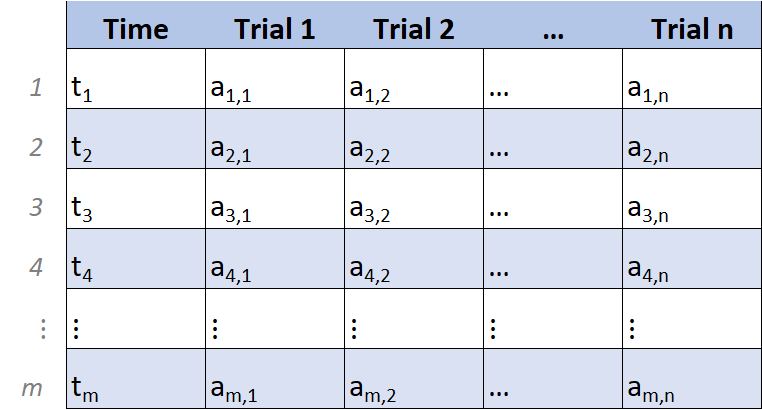
\includegraphics{./external_figures/fluoR_format_table_example.png}

\hypertarget{intro-examples}{%
\section{Examples}\label{intro-examples}}

\hypertarget{intro-formatdata}{%
\subsection{Format data}\label{intro-formatdata}}

Format the \texttt{GCaMP} dataset included with the fluoR package so the data is easier to work with.

\begin{Shaded}
\begin{Highlighting}[]
\KeywordTok{library}\NormalTok{(fluoR)}

\NormalTok{df <-}\StringTok{ }\KeywordTok{format_data}\NormalTok{(GCaMP)}
\KeywordTok{head}\NormalTok{(df)}
\end{Highlighting}
\end{Shaded}

\begin{verbatim}
##      Time Trial1 Trial2 Trial3 Trial4 Trial5 Trial6 Trial7 Trial8 Trial9
## 1 -3.9902 82.689 82.858 81.709 89.747 90.788 90.365 123.53 120.39 119.95
## 2 -3.9803 82.656 82.922 81.702 89.637 90.847 90.418 123.30 120.41 119.82
## 3 -3.9705 82.650 82.984 81.713 89.545 90.927 90.485 123.13 120.45 119.73
## 4 -3.9607 82.671 83.042 81.726 89.476 91.003 90.578 123.02 120.52 119.66
## 5 -3.9508 82.712 83.085 81.732 89.428 91.056 90.696 122.96 120.59 119.62
## 6 -3.9410 82.757 83.116 81.714 89.397 91.080 90.833 122.95 120.66 119.60
##   Trial10
## 1  116.94
## 2  116.97
## 3  117.00
## 4  117.01
## 5  117.00
## 6  116.97
\end{verbatim}

\hypertarget{stand}{%
\chapter{Standardizing Data}\label{stand}}

\begin{Shaded}
\begin{Highlighting}[]
\KeywordTok{library}\NormalTok{(fluoR)}
\NormalTok{df <-}\StringTok{ }\KeywordTok{format_data}\NormalTok{(GCaMP)}
\end{Highlighting}
\end{Shaded}

\hypertarget{stand-reasons}{%
\section{Reasons to standardize data}\label{stand-reasons}}

There are a few reasons to standardize your data before exploring your data.

1. Signal differs between subjects

\begin{itemize}
\tightlist
\item
  Regardless of the specific technologies used, there is almost always differences in signal strength for each subject
\end{itemize}

2. Signal differs between trials

\begin{itemize}
\tightlist
\item
  The strength of recording signal tends to decay over time
\end{itemize}

3. Utilizing baseline values

\begin{itemize}
\tightlist
\item
  Using transformations such as percent change allows you to center the data at an objective value
\item
  After centering your trial and post-trial data, the data is interpreted as relative to baseline values
\item
  The baseline period is typically assumed to be a ``resting'' period prior to exposure to the experimental manipulation. This means that using standardization methods (particularly z-scores) also takes baseline deviations into consideration.
\end{itemize}

\hypertarget{stand-methods}{%
\section{Methods of standardization}\label{stand-methods}}

A little alteration in how we compute z-scores can make a significant difference.

\hypertarget{stand-methods-zscore}{%
\subsection{z-scores}\label{stand-methods-zscore}}

Standard z-score transformations work the same way with time series data as with any other. The formula:

\begin{enumerate}
\def\labelenumi{\arabic{enumi}.}
\tightlist
\item
  centers every value (x) at the mean of the full time series (mu)
\item
  divides it by the standard deviation of the full time series (sigma).
\end{enumerate}

\begin{gather*}
  z_{i} = \frac{x_{i}-\mu}{\sigma}
\end{gather*}
\begin{align*}
  \text{where...} \\
  \mu &= \text{mean of population,} \\
  \sigma &= \text{standard deviation of population} \\
\end{align*}

This results in the same time series in terms of standard deviations from the mean, all in the context of the full time series.

\hypertarget{stand-methods-zscore-code}{%
\subsubsection{R Code}\label{stand-methods-zscore-code}}

\begin{Shaded}
\begin{Highlighting}[]
\NormalTok{z.scores <-}\StringTok{ }\KeywordTok{z_score}\NormalTok{(}\DataTypeTok{xvals =}\NormalTok{ df}\OperatorTok{$}\NormalTok{Trial8,}
                    \DataTypeTok{mu =} \KeywordTok{mean}\NormalTok{(df}\OperatorTok{$}\NormalTok{Trial8), }\CommentTok{# manual input of mu/sigma optional;}
                    \DataTypeTok{sigma =} \KeywordTok{sd}\NormalTok{(df}\OperatorTok{$}\NormalTok{Trial8)) }\CommentTok{# used for example purposes}
\end{Highlighting}
\end{Shaded}

\hypertarget{stand-methods-zscore-vis}{%
\subsubsection{Visualization}\label{stand-methods-zscore-vis}}

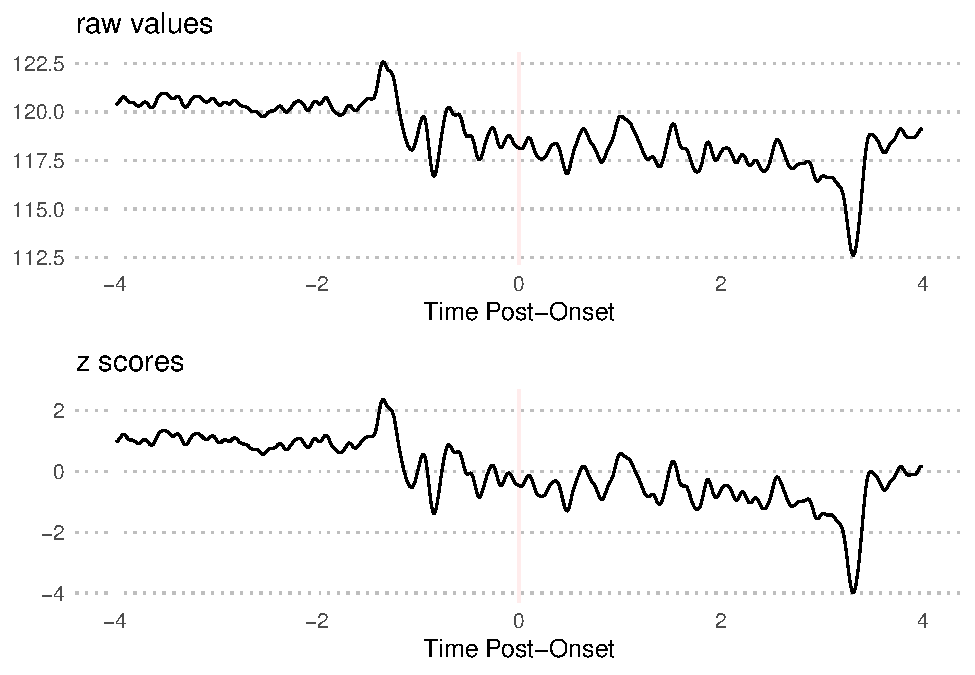
\includegraphics{fluoR_bookdown_files/figure-latex/unnamed-chunk-7-1.pdf}

\hypertarget{stand-methods-bzscore}{%
\subsection{baseline z-scores}\label{stand-methods-bzscore}}

Using the pre-event baseline period as the input values for computing z-scores can be useful in revealing changes in neural activity that you may not find by just comparing pre-trial and trial periods. This is in part because baseline periods tend to have relatively low variability.

As you can see from the formula, a lower standard deviation will increase positive values and decrease negative values - thus making changes in neural activity more apparent.

\begin{gather*}
  baseline \ z_{i} = \frac{x_{i}-\bar{x}_{baseline}}{s_{baseline}}
\end{gather*}
\begin{align*}
  \text{where...} \\
  \bar{x}_{baseline} &= \text{mean of values from baseline period,} \\
  {s}_{baseline} &= \text{standard deviation of values from baseline period} \\
\end{align*}

This results in a time series interpreted in terms of standard deviations and mean during the baseline period. Baseline z-scores are conceptually justifiable because the standard deviation is then the number of deviations from the mean when a subject is at rest. The values outside of the baseline period will be different using this version, but not within the baseline period.

\hypertarget{stand-methods-bzscore-code}{%
\subsubsection{R Code}\label{stand-methods-bzscore-code}}

\begin{Shaded}
\begin{Highlighting}[]
\CommentTok{### Extract baseline values}
\NormalTok{baseline.vals <-}\StringTok{ }\NormalTok{df}\OperatorTok{$}\NormalTok{Trial8[df}\OperatorTok{$}\NormalTok{Time }\OperatorTok{>=}\StringTok{ }\DecValTok{-4} \OperatorTok{&}\StringTok{ }\NormalTok{df}\OperatorTok{$}\NormalTok{Time }\OperatorTok{<=}\StringTok{ }\DecValTok{0}\NormalTok{]}

\CommentTok{### Compute z-scores}
\NormalTok{z.scores.baseline <-}\StringTok{ }\KeywordTok{z_score}\NormalTok{(}\DataTypeTok{xvals =}\NormalTok{ df}\OperatorTok{$}\NormalTok{Trial8,}
                             \DataTypeTok{mu =} \KeywordTok{mean}\NormalTok{(baseline.vals),}
                             \DataTypeTok{sigma =} \KeywordTok{sd}\NormalTok{(baseline.vals))}
\end{Highlighting}
\end{Shaded}

\hypertarget{stand-methods-bzscore-vis}{%
\subsubsection{Visualization}\label{stand-methods-bzscore-vis}}

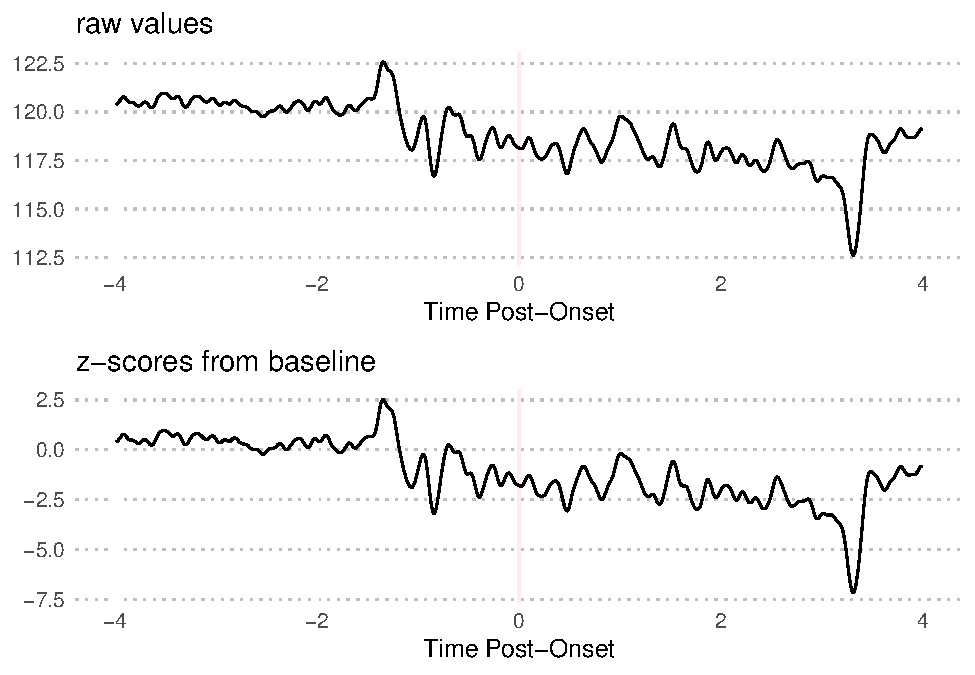
\includegraphics{fluoR_bookdown_files/figure-latex/unnamed-chunk-10-1.pdf}

\hypertarget{stand-methods-mzscore}{%
\subsection{modified z scores}\label{stand-methods-mzscore}}

Waveform data fluctuates naturally. But in the event of a change in activity due to external stimuli, signal variation tends to rapidly increase and/or decrease and becomes unruly.

\begin{gather*}
  modified \ z_{i} = \frac{0.6745(x_{i}-\widetilde{x})}{MAD}
\end{gather*}
\begin{align*}
  \text{where...} \\
  \widetilde{x} &= \text{sample median,} \\
  {MAD} &= \text{median absolute deviation}
\end{align*}

\hypertarget{stand-methods-mzscore-code}{%
\subsubsection{R Code}\label{stand-methods-mzscore-code}}

\begin{Shaded}
\begin{Highlighting}[]
\NormalTok{z.scores.modified <-}\StringTok{ }\KeywordTok{z_score}\NormalTok{(}\DataTypeTok{xvals =}\NormalTok{ df}\OperatorTok{$}\NormalTok{Trial8, }
                             \DataTypeTok{z.type =} \StringTok{'modified'}\NormalTok{)}
\end{Highlighting}
\end{Shaded}

\hypertarget{stand-methods-mzscore-vis}{%
\subsubsection{Visualization}\label{stand-methods-mzscore-vis}}

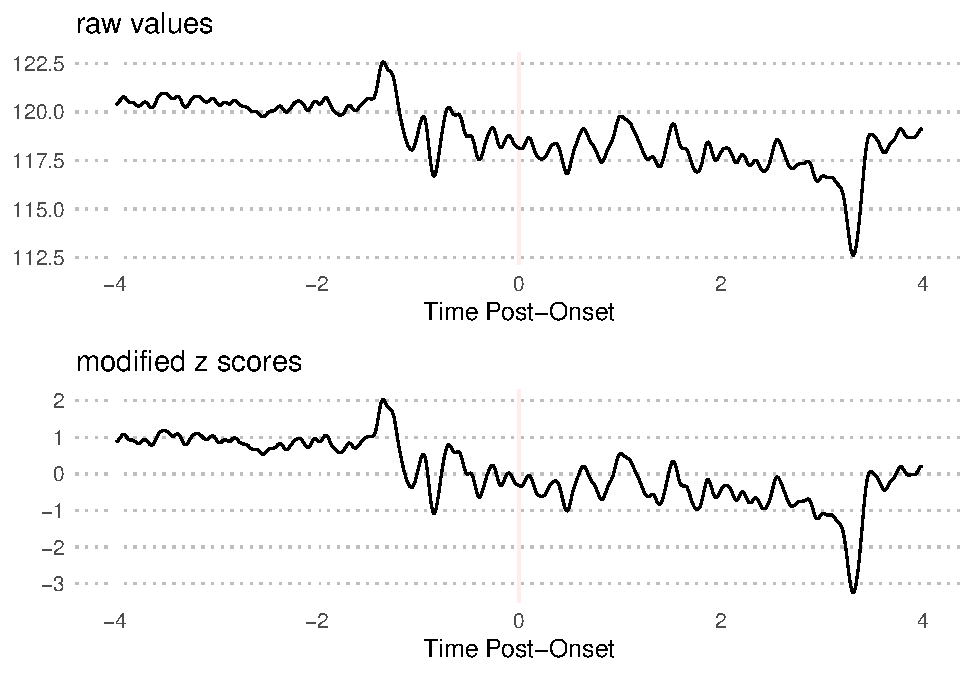
\includegraphics{fluoR_bookdown_files/figure-latex/unnamed-chunk-13-1.pdf}

\hypertarget{stand-comparison}{%
\section{z-score comparison}\label{stand-comparison}}

\hypertarget{stand-comparison-vis}{%
\subsection{Visualization}\label{stand-comparison-vis}}

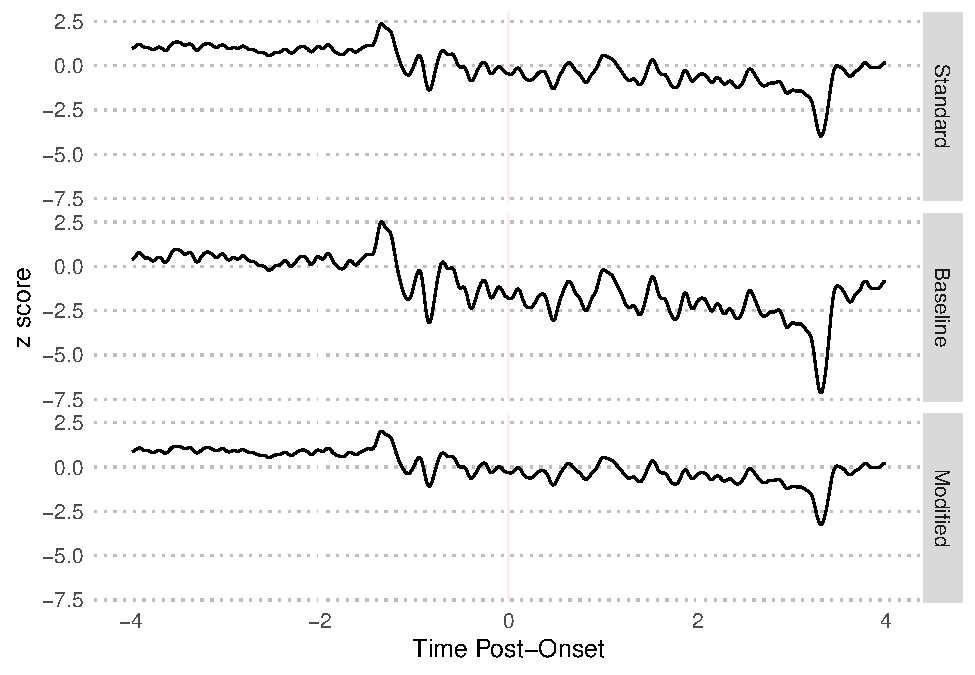
\includegraphics{fluoR_bookdown_files/figure-latex/unnamed-chunk-15-1.pdf}

\hypertarget{stand-comparison-table}{%
\subsection{Summary table}\label{stand-comparison-table}}

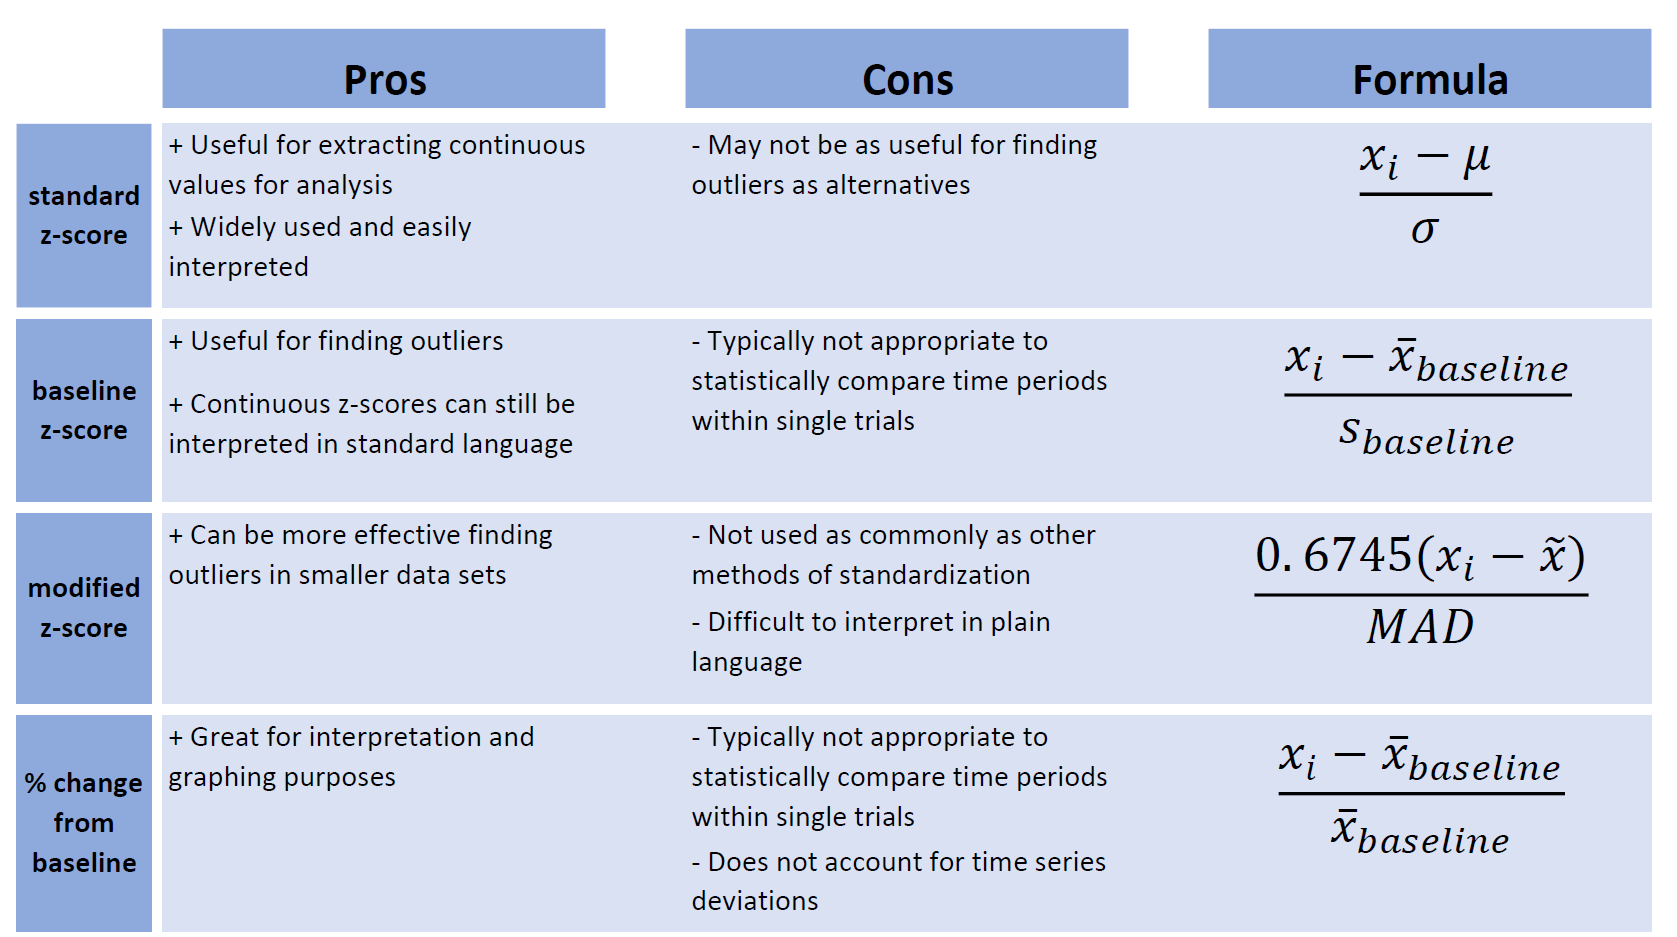
\includegraphics{./external_figures/tables/standardization_table.png}

\hypertarget{stand-examples}{%
\section{Examples}\label{stand-examples}}

\hypertarget{stand-examples-ex1}{%
\subsection{Example 1}\label{stand-examples-ex1}}

Standardize trial 8 so that the units are in terms of standard deviations from the mean of the full time series.

\begin{Shaded}
\begin{Highlighting}[]
\KeywordTok{z_score}\NormalTok{(}\DataTypeTok{xvals =}\NormalTok{ df}\OperatorTok{$}\NormalTok{Trial8,}
        \DataTypeTok{z.type =} \StringTok{'standard'}\NormalTok{)}
\end{Highlighting}
\end{Shaded}

\hypertarget{stand-examples-ex2}{%
\subsection{Example 2}\label{stand-examples-ex2}}

Standardize trial 8 so that the units are in terms of standard deviations from the mean of the pre-event period.

We can do this manually for each trial.

\begin{Shaded}
\begin{Highlighting}[]
\CommentTok{### Manual}
\NormalTok{baseline.vals <-}\StringTok{ }\NormalTok{df}\OperatorTok{$}\NormalTok{Trial8[df}\OperatorTok{$}\NormalTok{Time }\OperatorTok{>=}\StringTok{ }\DecValTok{-4} \OperatorTok{&}\StringTok{ }\NormalTok{df}\OperatorTok{$}\NormalTok{Time }\OperatorTok{<=}\StringTok{ }\DecValTok{0}\NormalTok{] }\CommentTok{# extract baseline values}
  
\NormalTok{baseline.z <-}\StringTok{ }\KeywordTok{z_score}\NormalTok{(}\DataTypeTok{xvals =}\NormalTok{ df}\OperatorTok{$}\NormalTok{Trial8,}
                      \DataTypeTok{mu =} \KeywordTok{mean}\NormalTok{(baseline.vals), }\CommentTok{# mean of baseline}
                      \DataTypeTok{sigma =} \KeywordTok{sd}\NormalTok{(baseline.vals), }\CommentTok{# sd of baseline}
                      \DataTypeTok{z.type =} \StringTok{'standard'}\NormalTok{)}
\end{Highlighting}
\end{Shaded}

Or we can use the \texttt{baseline\_transform} wrapper.

\begin{Shaded}
\begin{Highlighting}[]
\NormalTok{baseline.zdf <-}\StringTok{ }\KeywordTok{baseline_transform}\NormalTok{(}\DataTypeTok{dataframe =}\NormalTok{ df,}
                                   \DataTypeTok{trials =} \DecValTok{8}\NormalTok{,}
                                   \DataTypeTok{baseline.times =} \KeywordTok{c}\NormalTok{(}\OperatorTok{-}\DecValTok{4}\NormalTok{, }\DecValTok{0}\NormalTok{),}
                                   \DataTypeTok{type =} \StringTok{'z_standard'}\NormalTok{)}
\end{Highlighting}
\end{Shaded}

Both methods will result in the same values.

\begin{Shaded}
\begin{Highlighting}[]
\KeywordTok{all}\NormalTok{(baseline.zdf}\OperatorTok{$}\NormalTok{Trial8 }\OperatorTok{-}\StringTok{ }\NormalTok{baseline.z }\OperatorTok{==}\StringTok{ }\DecValTok{0}\NormalTok{)}
\end{Highlighting}
\end{Shaded}

\begin{verbatim}
## [1] TRUE
\end{verbatim}

\hypertarget{stand-examples-ex3}{%
\subsection{Example 3}\label{stand-examples-ex3}}

Standardize trial 8 so that the units are in terms of deviations from the median of the full time series.

\begin{Shaded}
\begin{Highlighting}[]
\KeywordTok{z_score}\NormalTok{(}\DataTypeTok{xvals =}\NormalTok{ df}\OperatorTok{$}\NormalTok{Trial8,}
        \DataTypeTok{z.type =} \StringTok{'modified'}\NormalTok{)}
\end{Highlighting}
\end{Shaded}

\hypertarget{stand-examples-ex4}{%
\subsection{Example 4}\label{stand-examples-ex4}}

Convert trial 8 so that the units are in terms of percent change from the mean of the pre-event period.

We can do this manually for each trial.

\begin{Shaded}
\begin{Highlighting}[]
\CommentTok{### Manual}
\NormalTok{baseline.vals <-}\StringTok{ }\NormalTok{df}\OperatorTok{$}\NormalTok{Trial8[df}\OperatorTok{$}\NormalTok{Time }\OperatorTok{>=}\StringTok{ }\DecValTok{-4} \OperatorTok{&}\StringTok{ }\NormalTok{df}\OperatorTok{$}\NormalTok{Time }\OperatorTok{<=}\StringTok{ }\DecValTok{0}\NormalTok{] }\CommentTok{# extract baseline values}
  
\NormalTok{perc.change <-}\StringTok{ }\KeywordTok{percent_change}\NormalTok{(}\DataTypeTok{xvals =}\NormalTok{ df}\OperatorTok{$}\NormalTok{Trial8,}
                              \DataTypeTok{base.val =} \KeywordTok{mean}\NormalTok{(baseline.vals))}
\end{Highlighting}
\end{Shaded}

Or we can use the \texttt{baseline\_transform} wrapper.

\begin{Shaded}
\begin{Highlighting}[]
\NormalTok{perc.changedf <-}\StringTok{ }\KeywordTok{baseline_transform}\NormalTok{(}\DataTypeTok{dataframe =}\NormalTok{ df,}
                                    \DataTypeTok{trials =} \DecValTok{8}\NormalTok{,}
                                    \DataTypeTok{baseline.times =} \KeywordTok{c}\NormalTok{(}\OperatorTok{-}\DecValTok{4}\NormalTok{, }\DecValTok{0}\NormalTok{),}
                                    \DataTypeTok{type =} \StringTok{'percent_change'}\NormalTok{)}
\end{Highlighting}
\end{Shaded}

Both methods will result in the same values.

\begin{Shaded}
\begin{Highlighting}[]
\KeywordTok{all}\NormalTok{(perc.changedf}\OperatorTok{$}\NormalTok{Trial8 }\OperatorTok{-}\StringTok{ }\NormalTok{perc.change }\OperatorTok{==}\StringTok{ }\DecValTok{0}\NormalTok{)}
\end{Highlighting}
\end{Shaded}

\begin{verbatim}
## [1] TRUE
\end{verbatim}

\hypertarget{vis}{%
\chapter{Visualization}\label{vis}}

\begin{Shaded}
\begin{Highlighting}[]
\KeywordTok{library}\NormalTok{(fluoR)}
\NormalTok{df <-}\StringTok{ }\KeywordTok{format_data}\NormalTok{(GCaMP)}
\end{Highlighting}
\end{Shaded}

\hypertarget{vis-multiple}{%
\section{Multiple trials}\label{vis-multiple}}

The \texttt{plot\_trials} command uses R's base plotting functions for data exploration purposes. Some benefits of using this function are:

\begin{enumerate}
\def\labelenumi{\arabic{enumi}.}
\tightlist
\item
  Much faster graphing than alternatives (e.g.~ggplot2, plotly)
\item
  Automatic scaling of x- and y- axes for graphing multiple trials so that all data points fit in the plot boundaries
\item
  Automatic color coding and trial number labeling
\item
  Plotting multiple trials with a single command while using default fluoR data frame format
\end{enumerate}

The more you need to graph your data in R, the more clear the tradeoff between \texttt{plot\_trials} and \texttt{ggplot} becomes.

\begin{itemize}
\tightlist
\item
  \texttt{plot\_trials} will save significant time from extra data manipulation when looking through your data, especially when examining a large number of trials
\item
  \texttt{ggplot} will be much more appropriate for publication and presentation graphing
\end{itemize}

\hypertarget{vis-multiple-plotfluor}{%
\subsection{plot\_trials}\label{vis-multiple-plotfluor}}

\begin{Shaded}
\begin{Highlighting}[]
\NormalTok{base.trials <-}\StringTok{ }\KeywordTok{plot_trials}\NormalTok{(}\DataTypeTok{dataframe =}\NormalTok{ df,}
                           \DataTypeTok{trials =} \DecValTok{8}\OperatorTok{:}\DecValTok{10}\NormalTok{)}
\end{Highlighting}
\end{Shaded}

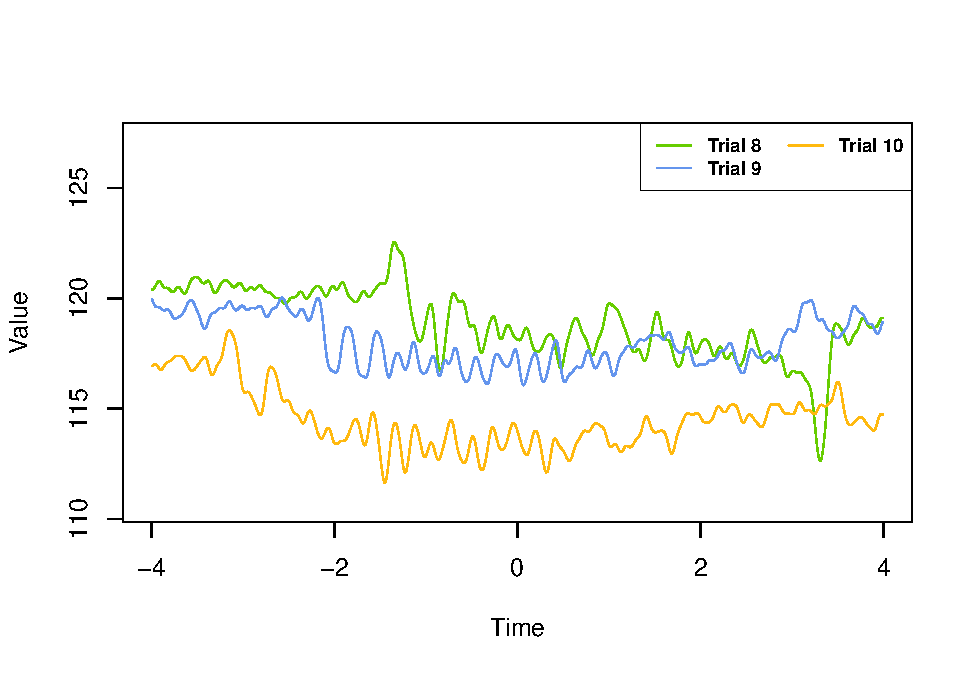
\includegraphics{fluoR_bookdown_files/figure-latex/unnamed-chunk-25-1.pdf}

\hypertarget{vis-multiple-plotgg}{%
\subsection{ggplot2}\label{vis-multiple-plotgg}}

For plotting multiple trials using ggplot2, we will need the data frame to be in ``long'' format. So, we stack the trials we want to plot.

\begin{Shaded}
\begin{Highlighting}[]
\NormalTok{df.long <-}\StringTok{ }\KeywordTok{data.frame}\NormalTok{(}
  \DataTypeTok{Time =} \KeywordTok{rep}\NormalTok{(df}\OperatorTok{$}\NormalTok{Time, }\DataTypeTok{times =} \DecValTok{3}\NormalTok{), }\CommentTok{# repeat time values by number of trials}
  \DataTypeTok{Values =} \KeywordTok{c}\NormalTok{(df}\OperatorTok{$}\NormalTok{Trial8, df}\OperatorTok{$}\NormalTok{Trial9, df}\OperatorTok{$}\NormalTok{Trial10), }\CommentTok{# vector of trial values}
  \DataTypeTok{Trial =} \KeywordTok{c}\NormalTok{(}\KeywordTok{rep}\NormalTok{(}\StringTok{"8"}\NormalTok{, }\KeywordTok{length}\NormalTok{(df}\OperatorTok{$}\NormalTok{Trial8)), }\CommentTok{# label trial numbers}
            \KeywordTok{rep}\NormalTok{(}\StringTok{"9"}\NormalTok{, }\KeywordTok{length}\NormalTok{(df}\OperatorTok{$}\NormalTok{Trial9)), }
            \KeywordTok{rep}\NormalTok{(}\StringTok{"10"}\NormalTok{, }\KeywordTok{length}\NormalTok{(df}\OperatorTok{$}\NormalTok{Trial10)))}
\NormalTok{)}
\end{Highlighting}
\end{Shaded}

Now we can make the graph using ggplot2.

\begin{Shaded}
\begin{Highlighting}[]
\KeywordTok{library}\NormalTok{(ggplot2)}
\KeywordTok{library}\NormalTok{(ggpubr) }\CommentTok{# for theme}

\KeywordTok{ggplot}\NormalTok{(df.long) }\OperatorTok{+}
\StringTok{  }\KeywordTok{geom_line}\NormalTok{(}\KeywordTok{aes}\NormalTok{(}\DataTypeTok{x =}\NormalTok{ Time, }\DataTypeTok{y =}\NormalTok{ Values,}
                \DataTypeTok{color =}\NormalTok{ Trial)) }\OperatorTok{+}
\StringTok{  }\KeywordTok{scale_color_manual}\NormalTok{(}\DataTypeTok{values =} \KeywordTok{c}\NormalTok{(}\StringTok{"8"}\NormalTok{ =}\StringTok{ 'chartreuse3'}\NormalTok{, }
                                \StringTok{"9"}\NormalTok{ =}\StringTok{ 'cornflowerblue'}\NormalTok{, }
                                \StringTok{"10"}\NormalTok{ =}\StringTok{ 'darkgoldenrod1'}\NormalTok{)) }\OperatorTok{+}
\StringTok{  }\KeywordTok{theme_pubclean}\NormalTok{()}
\end{Highlighting}
\end{Shaded}

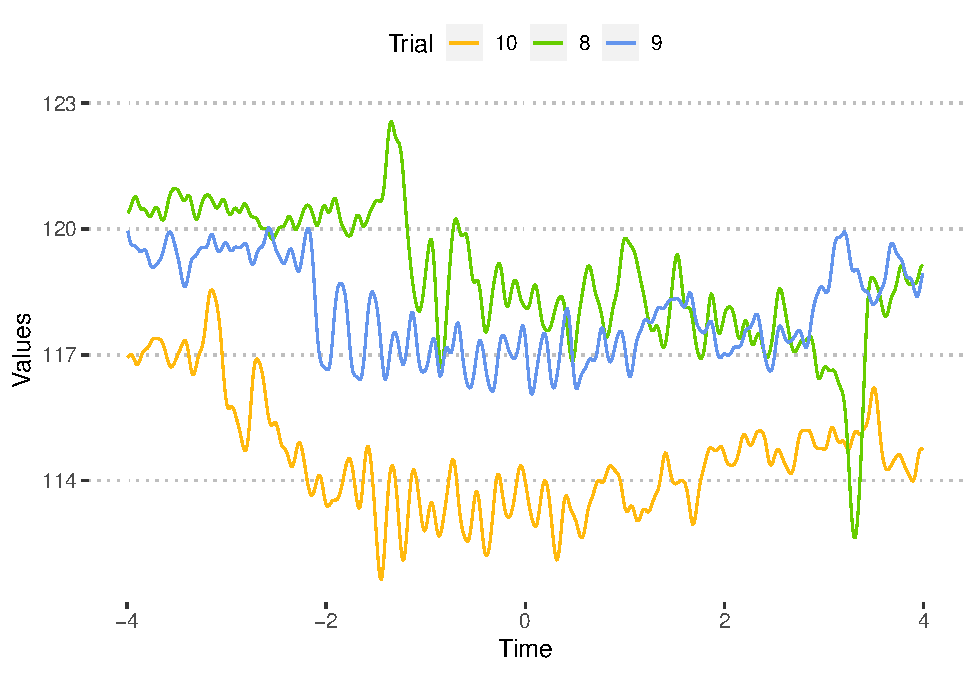
\includegraphics{fluoR_bookdown_files/figure-latex/unnamed-chunk-27-1.pdf}

\hypertarget{vis-ranges}{%
\section{Trial ranges}\label{vis-ranges}}

Let's say that you have 30 trials. As part of your hypothesis, you believe that neural activity will change shortly after exposure to a stimulus during trials 1-10, but not subsequent ones.

One method of examining this could be:

\begin{enumerate}
\def\labelenumi{\arabic{enumi}.}
\tightlist
\item
  Standardize your data so it accounts for within-subject and between-trial differences
\item
  Break your data into ``blocks'' of 10 and collapse the data across trials for each time point using a summary statistic such as the mean or median
\item
  Plot the values using 3 groups: trials 1-10, trials 11-20, and trials 21-30
\end{enumerate}

Unfortunately, a 30+ trial dataset would not be ideal to include in the fluoR package. So, we will use trial ``blocks'' of 3, which results in the groups being trials 1-3, 4-6, and 7-9.

For the first part, we standardize the data into z-scores from baseline.

\begin{Shaded}
\begin{Highlighting}[]
\CommentTok{### 1. Standardize data}
\NormalTok{df.stand <-}\StringTok{ }\KeywordTok{baseline_transform}\NormalTok{(}\DataTypeTok{dataframe =}\NormalTok{ df, }
                               \DataTypeTok{trials =} \DecValTok{1}\OperatorTok{:}\DecValTok{10}\NormalTok{, }
                               \DataTypeTok{baseline.times =} \KeywordTok{c}\NormalTok{(}\OperatorTok{-}\DecValTok{4}\NormalTok{,}\DecValTok{0}\NormalTok{),}
                               \DataTypeTok{type =} \StringTok{'z_standard'}\NormalTok{)}
\end{Highlighting}
\end{Shaded}

For the second part, we find the median value for each time point from each of the 3 trial blocks.

\begin{Shaded}
\begin{Highlighting}[]
\CommentTok{### 2. Summarize/collapse across blocks of trials}
\NormalTok{df.block1 <-}\StringTok{ }\KeywordTok{summarize_trials}\NormalTok{(}\DataTypeTok{dataframe =}\NormalTok{ df.stand, }\DataTypeTok{trials =} \DecValTok{1}\OperatorTok{:}\DecValTok{3}\NormalTok{,}
                              \DataTypeTok{summary.type =} \StringTok{'median'}\NormalTok{)}
\NormalTok{df.block2 <-}\StringTok{ }\KeywordTok{summarize_trials}\NormalTok{(}\DataTypeTok{dataframe =}\NormalTok{ df.stand, }\DataTypeTok{trials =} \DecValTok{4}\OperatorTok{:}\DecValTok{6}\NormalTok{,}
                              \DataTypeTok{summary.type =} \StringTok{'median'}\NormalTok{)}
\NormalTok{df.block3 <-}\StringTok{ }\KeywordTok{summarize_trials}\NormalTok{(}\DataTypeTok{dataframe =}\NormalTok{ df.stand, }\DataTypeTok{trials =} \DecValTok{7}\OperatorTok{:}\DecValTok{9}\NormalTok{,}
                              \DataTypeTok{summary.type =} \StringTok{'median'}\NormalTok{)}
\end{Highlighting}
\end{Shaded}

Graphing summarize data tends to be more for publication than exploration purposes, so we want to use ggplot2. Fortunately, creating multiple data frames \texttt{summarize\_trials} allows us to simply assign a label column to each data frame and combine them before graphing.

\begin{Shaded}
\begin{Highlighting}[]
\NormalTok{df.block1}\OperatorTok{$}\NormalTok{trial.range <-}\StringTok{ '1-3'}
\NormalTok{df.block2}\OperatorTok{$}\NormalTok{trial.range <-}\StringTok{ '4-6'}
\NormalTok{df.block3}\OperatorTok{$}\NormalTok{trial.range <-}\StringTok{ '7-9'}

\NormalTok{df.blocked <-}\StringTok{ }\KeywordTok{rbind}\NormalTok{(df.block1, df.block2, df.block3)}
\end{Highlighting}
\end{Shaded}

Last, we plot the summarized values.

\begin{Shaded}
\begin{Highlighting}[]
\KeywordTok{ggplot}\NormalTok{(df.blocked) }\OperatorTok{+}
\StringTok{  }\KeywordTok{geom_vline}\NormalTok{(}\DataTypeTok{xintercept =} \DecValTok{0}\NormalTok{,}
             \DataTypeTok{color =} \StringTok{'red'}\NormalTok{, }\DataTypeTok{alpha =} \FloatTok{0.075}\NormalTok{) }\OperatorTok{+}\StringTok{ }\CommentTok{# event onset at 0}
\StringTok{  }\KeywordTok{geom_line}\NormalTok{(}\KeywordTok{aes}\NormalTok{(}\DataTypeTok{x =}\NormalTok{ Time, }\DataTypeTok{y =}\NormalTok{ summ.trials,}
                \DataTypeTok{color =}\NormalTok{ trial.range)) }\OperatorTok{+}\StringTok{ }\CommentTok{# trial lines}
\StringTok{  }\KeywordTok{labs}\NormalTok{(}
    \DataTypeTok{x =} \StringTok{'Time Post-Onset'}\NormalTok{,}
    \DataTypeTok{y =} \StringTok{'z score'}\NormalTok{,}
    \DataTypeTok{color =} \StringTok{'Trials'}
\NormalTok{  ) }\OperatorTok{+}
\StringTok{  }\KeywordTok{theme_pubclean}\NormalTok{()}
\end{Highlighting}
\end{Shaded}

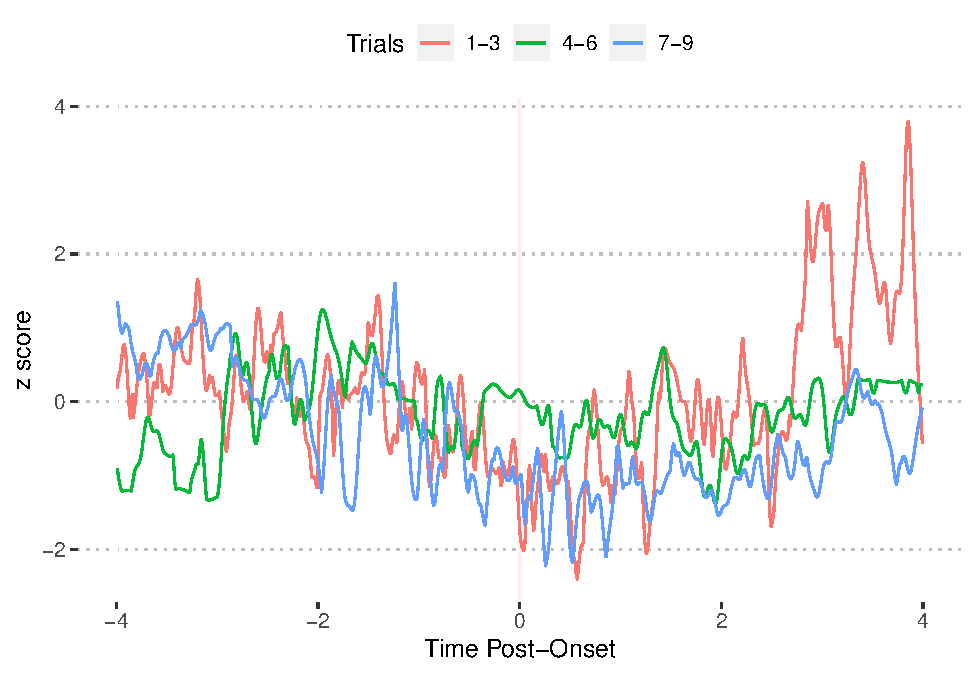
\includegraphics{fluoR_bookdown_files/figure-latex/unnamed-chunk-31-1.pdf}

\hypertarget{vis-smoothing}{%
\section{Smoothing}\label{vis-smoothing}}

As you can see by the previous graphs, the recorded data looks sharp when graphed across time points. While this should be used for the data extraction and analysis phase, we do not have this limitation when graphing.

The idea is to keep your data as similar as possible to the original time series while making an appealing visualization. Time series filters can help with this.

\hypertarget{vis-smoothing-whittaker}{%
\subsection{Whittaker filter}\label{vis-smoothing-whittaker}}

The Whittaker filter is a smoother that fits a curve to the data and penalizes highly-deviating points using the penalized least squares (PLS) method. There are two important parameters for this formula:

\begin{itemize}
\tightlist
\item
  lambda - smoothing parameter that controls the amount of curvature allowed for the least-squares fit. A smaller lambda permits more curvature
\item
  d - order of differences for the least-squares penalty
\end{itemize}

The \texttt{pracma} R package includes an implementation of the Whittaker smoother \citep{borchers_pracma_2019}.

\begin{Shaded}
\begin{Highlighting}[]
\KeywordTok{library}\NormalTok{(pracma)}

\NormalTok{Trial8.whittaker <-}\StringTok{ }\KeywordTok{whittaker}\NormalTok{(}\DataTypeTok{y =}\NormalTok{ df}\OperatorTok{$}\NormalTok{Trial8)}
\end{Highlighting}
\end{Shaded}

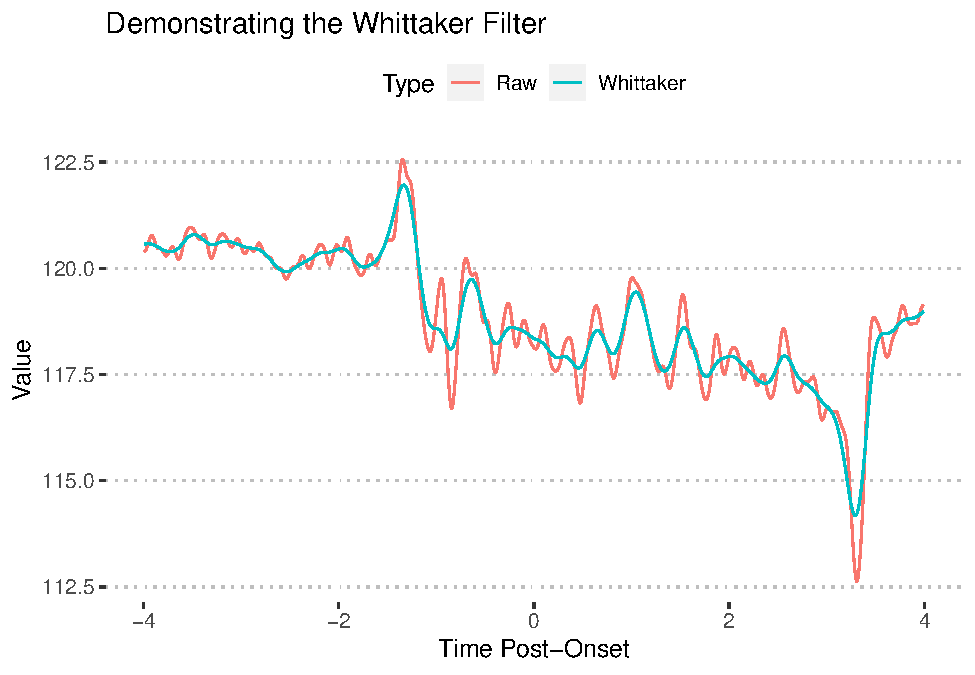
\includegraphics{fluoR_bookdown_files/figure-latex/unnamed-chunk-34-1.pdf}

As shown by the above figure, the Whittaker filter produces a much more ``tame'' line. In turn, the line makes extreme values (peaks and valleys) smaller. This filter tends to be useful when trying to smooth data without flattening too many curves.

\hypertarget{vis-smoothing-gam}{%
\subsection{Generalized additive modeling}\label{vis-smoothing-gam}}

I have only found generalized additive modeling useful as a smoother or for predictive modeling. This is because GAM's tend to overfit the model to the data, which is a big no-no in hypothesis testing.

The \texttt{mgcv} R package includes a popular implementation of GAM's. The formula input for the package's \texttt{gam} function is styled like R's base \texttt{glm} function. To smooth our time series data, we use Time as the dependent variable and our observation values as the independent variable.

\begin{Shaded}
\begin{Highlighting}[]
\CommentTok{### Compute gam}
\KeywordTok{library}\NormalTok{(mgcv)}

\CommentTok{### Construct model}
\NormalTok{gam1 <-}\StringTok{ }\KeywordTok{gam}\NormalTok{(Time }\OperatorTok{~}\StringTok{ }\KeywordTok{s}\NormalTok{(Trial8, }\DataTypeTok{bs =} \StringTok{'cs'}\NormalTok{), }\DataTypeTok{data =}\NormalTok{ df) }\CommentTok{# construct model}
\NormalTok{gamfit <-}\StringTok{ }\KeywordTok{predict}\NormalTok{(gam1, }\DataTypeTok{data =}\NormalTok{ df) }\CommentTok{# use model to create fitted line}
\end{Highlighting}
\end{Shaded}

There are also a handful of other parameters found in \href{https://www.rdocumentation.org/packages/mgcv/versions/1.8-33/topics/gam}{the documentation} that can be changed, but I typically avoid. If you don't need to change the additional parameters, \texttt{ggplot2} has a command that smooths the data automatically and scales it to your original data points.

\begin{Shaded}
\begin{Highlighting}[]
\KeywordTok{ggplot}\NormalTok{(df, }\KeywordTok{aes}\NormalTok{(}\DataTypeTok{x =}\NormalTok{ Time, }\DataTypeTok{y =}\NormalTok{ Trial8)) }\OperatorTok{+}
\StringTok{  }\KeywordTok{geom_line}\NormalTok{() }\OperatorTok{+}
\StringTok{  }\KeywordTok{stat_smooth}\NormalTok{(}\DataTypeTok{method =} \StringTok{'gam'}\NormalTok{) }\OperatorTok{+}
\StringTok{  }\KeywordTok{labs}\NormalTok{(}
    \DataTypeTok{x =} \StringTok{'Time Post-Offset'}\NormalTok{,}
    \DataTypeTok{y =} \StringTok{'Value'}\NormalTok{,}
    \DataTypeTok{title =} \StringTok{'GAM smoothed line over raw values'}
\NormalTok{    ) }\OperatorTok{+}
\StringTok{  }\KeywordTok{theme_pubclean}\NormalTok{()}
\end{Highlighting}
\end{Shaded}

\begin{verbatim}
## `geom_smooth()` using formula 'y ~ s(x, bs = "cs")'
\end{verbatim}

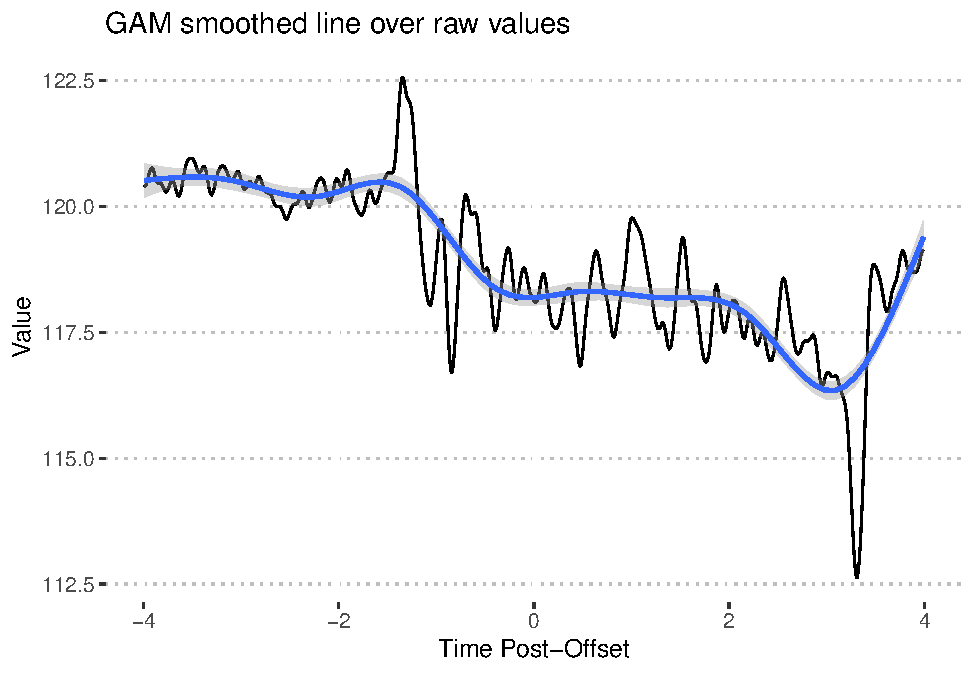
\includegraphics{fluoR_bookdown_files/figure-latex/unnamed-chunk-36-1.pdf}

In this situation, the GAM captures the general direction of the data points but almost completely removes smaller peaks/valleys and flattens extreme values.

\hypertarget{vis-smoothing-loess}{%
\subsection{Loess}\label{vis-smoothing-loess}}

\hypertarget{vis-smoothing-loess-model}{%
\subsubsection{model}\label{vis-smoothing-loess-model}}

Locally estimated scatterplot smoothing (loess) is a non-parametric regression that uses multiple regression in k-nearest-neighbor meta-models.

Loess models require much more data than standard regression. Luckily, this makes loess a solid choice for smoothing fiber photometry data. Much less so for testing hypotheses.

The \texttt{stats} package includes the \texttt{loess} function that allows us to implement it in typical R regression form. However, researchers will seldom find use for loess as a model itself.

\begin{Shaded}
\begin{Highlighting}[]
\KeywordTok{ggplot}\NormalTok{(df, }\KeywordTok{aes}\NormalTok{(}\DataTypeTok{x =}\NormalTok{ Time, }\DataTypeTok{y =}\NormalTok{ Trial8)) }\OperatorTok{+}
\StringTok{  }\KeywordTok{geom_line}\NormalTok{() }\OperatorTok{+}
\StringTok{  }\KeywordTok{stat_smooth}\NormalTok{(}\DataTypeTok{method =} \StringTok{'loess'}\NormalTok{) }\OperatorTok{+}
\StringTok{  }\KeywordTok{labs}\NormalTok{(}
    \DataTypeTok{x =} \StringTok{'Time Post-Offset'}\NormalTok{,}
    \DataTypeTok{y =} \StringTok{'Value'}\NormalTok{,}
    \DataTypeTok{title =} \StringTok{'Loess smoothed line over raw values'}
\NormalTok{    ) }\OperatorTok{+}
\StringTok{  }\KeywordTok{theme_pubclean}\NormalTok{()}
\end{Highlighting}
\end{Shaded}

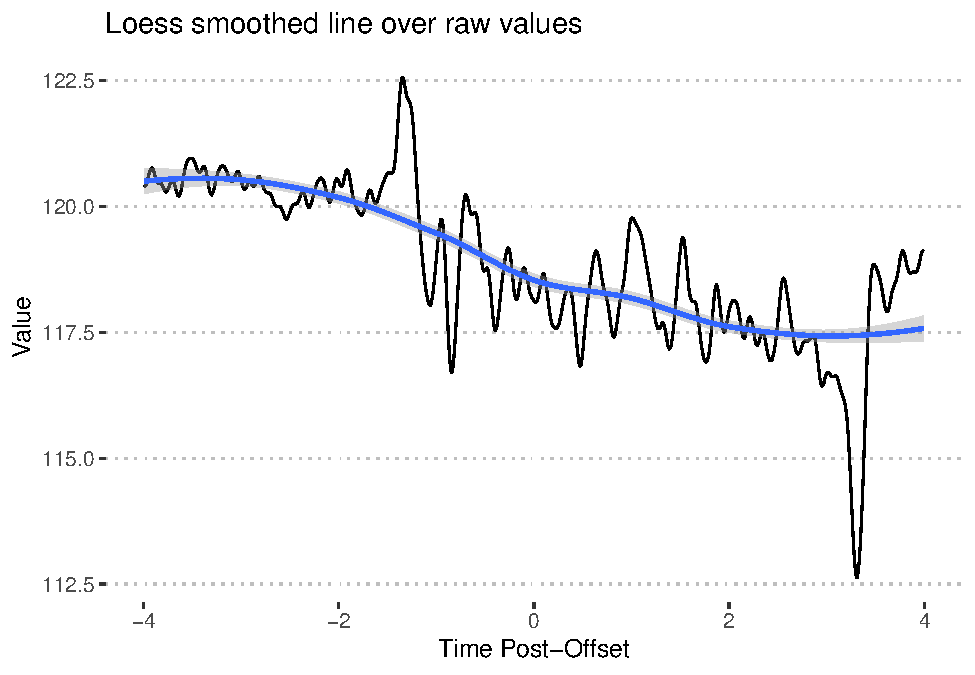
\includegraphics{fluoR_bookdown_files/figure-latex/unnamed-chunk-37-1.pdf}

Additionally, you can change the \texttt{span} parameter to control the degree of smoothing.

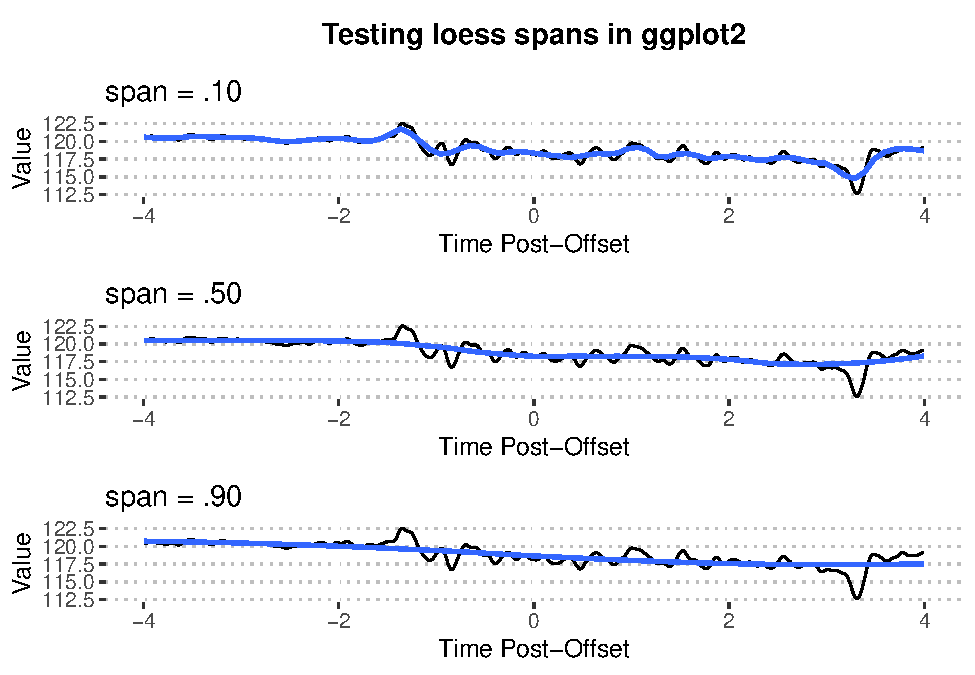
\includegraphics{fluoR_bookdown_files/figure-latex/unnamed-chunk-38-1.pdf}

\hypertarget{vis-furtherreading}{%
\section{Further reading}\label{vis-furtherreading}}

Programming

\begin{itemize}
\tightlist
\item
  UCLA's statistics consulting released a guide to working with time series smoothing using the \texttt{ggplot2} package \citep{ucla_smoothing}
\end{itemize}

Math

\begin{itemize}
\tightlist
\item
  \citep{wood_smoothing_2016} offer examples of time series smoothing using the \texttt{mgcv} package. The authors also go very in-depth with the math behind the methods.
\end{itemize}

\hypertarget{analysis}{%
\chapter{Analysis}\label{analysis}}

\begin{Shaded}
\begin{Highlighting}[]
\KeywordTok{library}\NormalTok{(fluoR)}
\KeywordTok{library}\NormalTok{(ggplot2)}
\KeywordTok{library}\NormalTok{(ggpubr)}
\KeywordTok{library}\NormalTok{(cowplot)}
\KeywordTok{theme_set}\NormalTok{(}\KeywordTok{theme_pubclean}\NormalTok{())}

\NormalTok{df <-}\StringTok{ }\KeywordTok{format_data}\NormalTok{(GCaMP)}
\end{Highlighting}
\end{Shaded}

\hypertarget{analysis-metrics}{%
\section{Metrics}\label{analysis-metrics}}

\hypertarget{analysis-metrics-peaks}{%
\subsection{Peaks}\label{analysis-metrics-peaks}}

Because of R's relative ease in subsetting data, I did not include a z-score filter in any of the functions.

\hypertarget{analysis-metrics-peaks-find}{%
\subsubsection{peak/valley finding}\label{analysis-metrics-peaks-find}}

\texttt{find\_peaks} from the \texttt{fluoR} package lets the user find peaks and valleys using a vector of numbers.

The \texttt{n.points} parameter is used to determine how many decreasing/increasing points on each side of a peak/valley are required for the point to be considered a peak or valley.

\hypertarget{analysis-metrics-peaks-find-peaks}{%
\paragraph{peaks}\label{analysis-metrics-peaks-find-peaks}}

Using a positive value for \texttt{find\_peaks} will return peaks

\begin{Shaded}
\begin{Highlighting}[]
\NormalTok{pks <-}\StringTok{ }\KeywordTok{find_peaks}\NormalTok{(}\DataTypeTok{xvals =}\NormalTok{ df}\OperatorTok{$}\NormalTok{Trial8,}
                  \DataTypeTok{n.points =} \DecValTok{10}\NormalTok{) }\CommentTok{# 10 decreasing points on each side}
\end{Highlighting}
\end{Shaded}

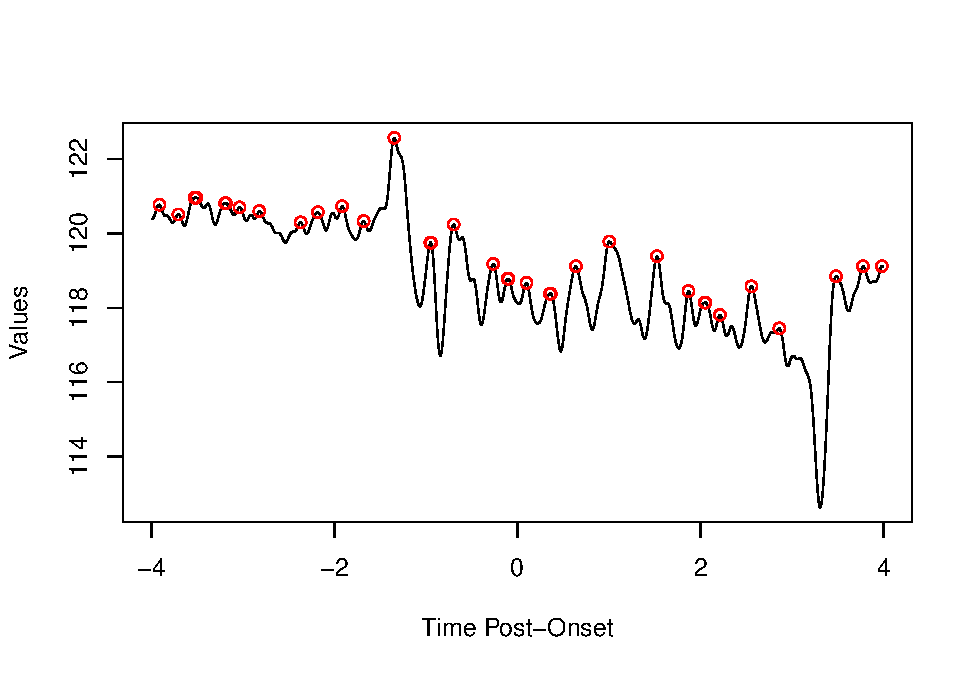
\includegraphics{fluoR_bookdown_files/figure-latex/unnamed-chunk-41-1.pdf}

\hypertarget{analysis-metrics-peaks-find-valleys}{%
\paragraph{peaks}\label{analysis-metrics-peaks-find-valleys}}

Using a negative value for \texttt{find\_peaks} will return valleys (lower extremes)

\begin{Shaded}
\begin{Highlighting}[]
\NormalTok{pks <-}\StringTok{ }\KeywordTok{find_peaks}\NormalTok{(}\DataTypeTok{xvals =}\NormalTok{ df}\OperatorTok{$}\NormalTok{Trial8,}
                  \DataTypeTok{n.points =} \DecValTok{-10}\NormalTok{) }\CommentTok{# 10 increasing points on each side}
\end{Highlighting}
\end{Shaded}

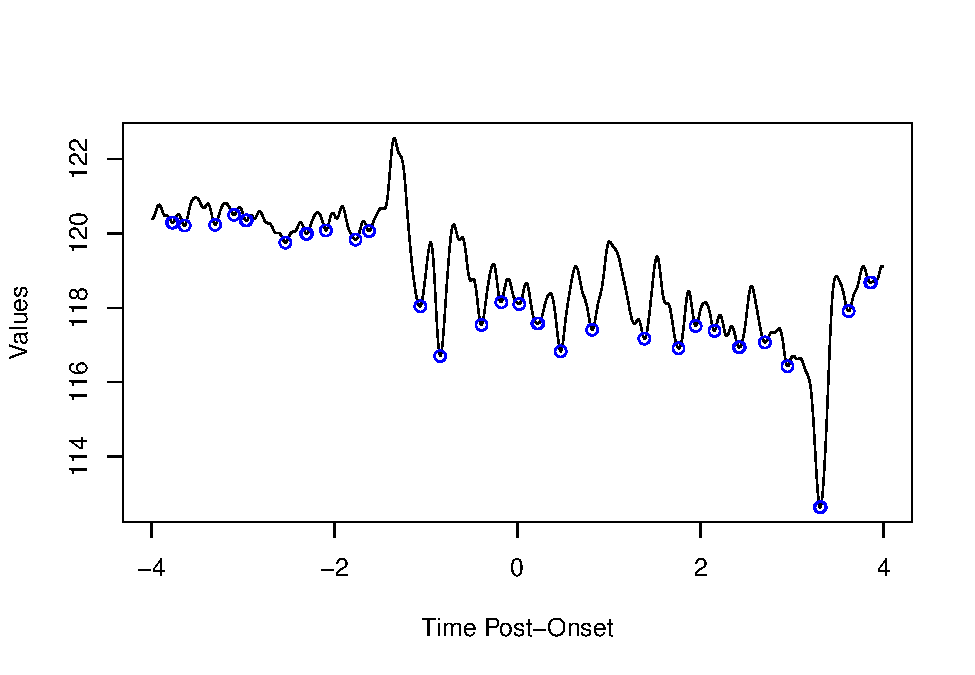
\includegraphics{fluoR_bookdown_files/figure-latex/unnamed-chunk-43-1.pdf}

\hypertarget{analysis-metrics-peaks-sensitivity}{%
\subsubsection{adjusting sensitivity}\label{analysis-metrics-peaks-sensitivity}}

The \texttt{n.points} parameter can be changed to prevent returning false positives.

\begin{Shaded}
\begin{Highlighting}[]
\NormalTok{pks5 <-}\StringTok{ }\KeywordTok{find_peaks}\NormalTok{(}\DataTypeTok{xvals =}\NormalTok{ df}\OperatorTok{$}\NormalTok{Trial8, }\DataTypeTok{n.points =} \DecValTok{5}\NormalTok{)}
\NormalTok{pks10 <-}\StringTok{ }\KeywordTok{find_peaks}\NormalTok{(}\DataTypeTok{xvals =}\NormalTok{ df}\OperatorTok{$}\NormalTok{Trial8, }\DataTypeTok{n.points =} \DecValTok{10}\NormalTok{)}
\NormalTok{pks20 <-}\StringTok{ }\KeywordTok{find_peaks}\NormalTok{(}\DataTypeTok{xvals =}\NormalTok{ df}\OperatorTok{$}\NormalTok{Trial8, }\DataTypeTok{n.points =} \DecValTok{20}\NormalTok{)}
\end{Highlighting}
\end{Shaded}

\begin{itemize}
\tightlist
\item
  \texttt{n.points\ =\ 5} returns the indices for 44 peaks
\item
  \texttt{n.points\ =\ 10} returns the indices for 34 peaks
\item
  \texttt{n.points\ =\ 20} returns the indices for 23 peaks
\end{itemize}

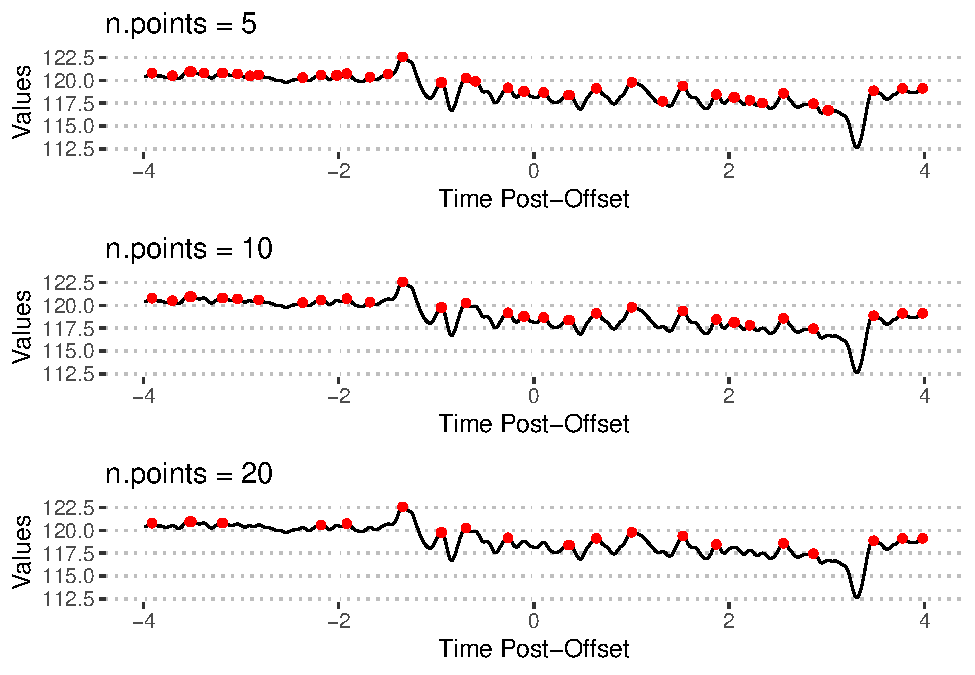
\includegraphics{fluoR_bookdown_files/figure-latex/unnamed-chunk-46-1.pdf}

\hypertarget{analysis-metrics-peaks-distance}{%
\subsubsection{distance between peaks}\label{analysis-metrics-peaks-distance}}

fluoR's \texttt{distance\_between\_peaks} function was written to extract values at each peak and between peaks for a single trial. This was inspired by the survival regression analysis done by \citep{gunaydin_natural_2014}.

\begin{Shaded}
\begin{Highlighting}[]
\NormalTok{peak.dist <-}\StringTok{ }\KeywordTok{distance_between_peaks}\NormalTok{(}\DataTypeTok{dataframe =}\NormalTok{ df,}
                                    \DataTypeTok{trial =} \DecValTok{8}\NormalTok{,}
                                    \DataTypeTok{time.range =} \KeywordTok{c}\NormalTok{(}\OperatorTok{-}\DecValTok{4}\NormalTok{,}\DecValTok{4}\NormalTok{),}
                                    \DataTypeTok{n.points =} \DecValTok{8}\NormalTok{)}
\KeywordTok{head}\NormalTok{(peak.dist)}
\end{Highlighting}
\end{Shaded}

\begin{verbatim}
##   index.start index.stop index.distance peak.diff.time peak1.intensity
## 1           9         30             21         0.2064          120.77
## 2          30         48             18         0.1770          120.51
## 3          48         50              2         0.0196          120.96
## 4          50         63             13         0.1278          120.96
## 5          63         82             19         0.1868          120.80
## 6          82         83              1         0.0098          120.81
##   peak2.intensity peak.diff.intensity
## 1          120.51               -0.26
## 2          120.96                0.45
## 3          120.96                0.00
## 4          120.80               -0.16
## 5          120.81                0.01
## 6          120.81                0.00
\end{verbatim}

The variables returned are useful for both graphing and analysis.

\begin{itemize}
\tightlist
\item
  \texttt{index.start} and \texttt{index.stop} for indexing in reference to the original dataframe
\item
  \texttt{index.distance} for discrete counts, regardless of how frequently data points are recorded
\item
  \texttt{peak.diff.time} for the time between each pair of peaks
\item
  \texttt{peak1.intensity} and \texttt{peak2.intensity} for the values each peak is located at (think counting peaks above a specific z score)
\item
  \texttt{peak.diff.intensity} for finding continuous increases or decreases in peak fluorescence signal over time
\end{itemize}

\hypertarget{analysis-metrics-auc}{%
\subsection{Area under curve}\label{analysis-metrics-auc}}

One may decide that it is best to capture the full area underneath a curve. Area under curve (AUC) allows us to combine x (Time) and y (Intensity) variables into one value.

There are three important points one should consider before using AUC as a metric for statistical comparisons:
- the length for each time period being compared should be equal (e.g.~2s pre-onset vs.~2s post-onset)
- the values should be standardized or centered within each trial (e.g.~z-scores from baseline)
- computing the AUC includes negative values, which can result in a negative value and is moderately affected by large outliers

fluoR includes the function \texttt{auc.pre} to quickly calculate the AUC for a range of trials during a specified period of time. As an example of how this can be used, let's compare full pre-trial and post-trial periods for trials 1-4.

\begin{Shaded}
\begin{Highlighting}[]
\CommentTok{### Pre-onset}
\NormalTok{auc.pre <-}\StringTok{ }\KeywordTok{auc_trials}\NormalTok{(}\DataTypeTok{dataframe =}\NormalTok{ df, }\DataTypeTok{trials =} \DecValTok{1}\OperatorTok{:}\DecValTok{4}\NormalTok{,}
                      \DataTypeTok{time.range =} \KeywordTok{c}\NormalTok{(}\OperatorTok{-}\DecValTok{4}\NormalTok{,}\DecValTok{0}\NormalTok{))}

\CommentTok{### Post-onset}
\NormalTok{auc.post <-}\StringTok{ }\KeywordTok{auc_trials}\NormalTok{(}\DataTypeTok{dataframe =}\NormalTok{ df, }\DataTypeTok{trials =} \DecValTok{1}\OperatorTok{:}\DecValTok{4}\NormalTok{,}
                       \DataTypeTok{time.range =} \KeywordTok{c}\NormalTok{(}\DecValTok{0}\NormalTok{,}\DecValTok{4}\NormalTok{))}

\KeywordTok{head}\NormalTok{(auc.pre)}
\end{Highlighting}
\end{Shaded}

\begin{verbatim}
##   Trial1   Trial2   Trial3   Trial4 
## 328.5656 329.6170 325.8933 361.4260
\end{verbatim}

\begin{Shaded}
\begin{Highlighting}[]
\KeywordTok{head}\NormalTok{(auc.post)}
\end{Highlighting}
\end{Shaded}

\begin{verbatim}
##   Trial1   Trial2   Trial3   Trial4 
## 328.5480 331.3686 329.9789 361.0577
\end{verbatim}

The function returns a named vector for each trial's AUC so we can compare AUC values within and between trials.

\hypertarget{analysis-app}{%
\section{Applications}\label{analysis-app}}

\hypertarget{analysis-app-numpeaks}{%
\subsection{Number of peaks above z score}\label{analysis-app-numpeaks}}

Regardless of the periods of time being compared, the first step of using this metric is to determine which peaks are significant. We can do this by using the \texttt{n.points} parameter with the \texttt{distance\_between\_peaks} function and a set number z-score cutoff. The idea is to make the best combination to represent measured behaviors without excessively skewing the data toward significant or non-significant results.

\begin{itemize}
\tightlist
\item
  judging by word of mouth from other researchers, ``significant'' peaks tend to be standard z scores of 1.96 and over. But this is not a strict cutoff. It can also be raised to avoid false positives.
\item
  the \texttt{n.points} step is a bit trickier and may require adjusting the parameter.
\end{itemize}

Note that this approach does not specifically represent increases in activity per wave. In other words, it quantifies peak points of fluorescence, not the amount of increase in fluorescence from the preceding valley.

\hypertarget{analysis-app-numpeaks-ex1}{%
\subsubsection{Example 1}\label{analysis-app-numpeaks-ex1}}

We first need to standardize the data so that the intensity values represent standard deviations from the baseline mean.

\begin{Shaded}
\begin{Highlighting}[]
\CommentTok{# transform to z-scores using pre-event period as baseline}
\NormalTok{df.stand <-}\StringTok{ }\KeywordTok{baseline_transform}\NormalTok{(}\DataTypeTok{dataframe =}\NormalTok{ df, }\DataTypeTok{trials =} \DecValTok{1}\OperatorTok{:}\DecValTok{8}\NormalTok{,}
                               \DataTypeTok{baseline.times =} \KeywordTok{c}\NormalTok{(}\OperatorTok{-}\DecValTok{4}\NormalTok{,}\DecValTok{0}\NormalTok{)) }
\end{Highlighting}
\end{Shaded}

Then, we need to determine criteria for the peaks. Here, we can use the following:

\begin{itemize}
\tightlist
\item
  peak (inflection) points 1.96 z scores and above
\item
  peaks must have 10 data points decreasing on each side to be considered ``significant''
\end{itemize}

To apply this method, is easiest to apply the \texttt{distance\_between\_peaks} function across trials using a loop. I plan to change this function in the future for automatic compatibility with multiple trials.

\begin{Shaded}
\begin{Highlighting}[]
\NormalTok{big.list <-}\StringTok{ }\KeywordTok{list}\NormalTok{() }\CommentTok{# holding list}
\NormalTok{trial.range <-}\StringTok{ }\DecValTok{1}\OperatorTok{:}\DecValTok{8}

\CommentTok{### Loop across trials}
\ControlFlowTok{for}\NormalTok{(i }\ControlFlowTok{in}\NormalTok{ trial.range)\{}
  \CommentTok{## find peaks}
\NormalTok{  df.pks <-}\StringTok{ }\KeywordTok{distance_between_peaks}\NormalTok{(}\DataTypeTok{dataframe =}\NormalTok{ df.stand, }\DataTypeTok{trial =}\NormalTok{ i,}
                                   \DataTypeTok{time.range =} \KeywordTok{c}\NormalTok{(}\DecValTok{0}\NormalTok{,}\DecValTok{4}\NormalTok{), }
                                   \DataTypeTok{n.points =} \DecValTok{10}\NormalTok{)}
  \CommentTok{## specify trial number}
  \CommentTok{## add if-else statement incase 0 peaks are returned}
  \ControlFlowTok{if}\NormalTok{(}\KeywordTok{nrow}\NormalTok{(df.pks) }\OperatorTok{>}\StringTok{ }\DecValTok{0}\NormalTok{)\{}
\NormalTok{    df.pks}\OperatorTok{$}\NormalTok{trial <-}\StringTok{ }\NormalTok{i}
\NormalTok{  \}}
  
  \CommentTok{## add to list}
\NormalTok{  big.list[[i]] <-}\StringTok{ }\NormalTok{df.pks}
\NormalTok{\}}

\CommentTok{### Combine list of data frames}
\NormalTok{df.peaks <-}\StringTok{ }\KeywordTok{do.call}\NormalTok{(rbind, big.list)}
\end{Highlighting}
\end{Shaded}

Now we have our data frame of information on peaks with 10 decreasing points on each side.

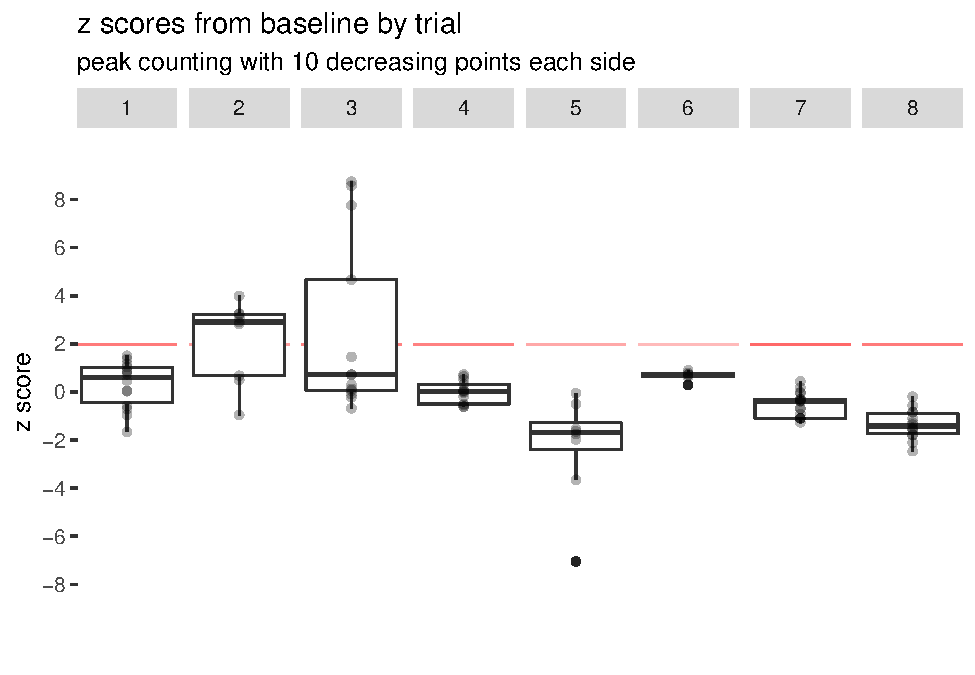
\includegraphics{fluoR_bookdown_files/figure-latex/unnamed-chunk-51-1.pdf}

It seems like only trials 2 and 3 had any post-event z scores above 1.96. Therefore, the fluorescence signal likely did not spike or increase for a significant number of times past baseline for 6 of 8 trials.

We can get the specific number of peaks that filled the z-score criteria as well. The \texttt{dplyr} package has a few functions that let us quickly compute counts by group.

\begin{Shaded}
\begin{Highlighting}[]
\KeywordTok{library}\NormalTok{(dplyr)}

\CommentTok{### Filter based on z score cutoff}
\NormalTok{df.peaks.filt <-}\StringTok{ }\NormalTok{df.peaks }\OperatorTok
\StringTok{  }\KeywordTok{filter}\NormalTok{(peak1.intensity }\OperatorTok{>}\StringTok{ }\FloatTok{1.96} \OperatorTok{|}\StringTok{ }\NormalTok{peak2.intensity }\OperatorTok{>}\StringTok{ }\FloatTok{1.96}\NormalTok{)}

\CommentTok{### Count values per trial}
\NormalTok{total.peaks <-}\StringTok{ }\NormalTok{df.peaks.filt }\OperatorTok
\StringTok{  }\KeywordTok{group_by}\NormalTok{(trial) }\OperatorTok
\StringTok{  }\KeywordTok{tally}\NormalTok{()}

\KeywordTok{print}\NormalTok{(total.peaks)}
\end{Highlighting}
\end{Shaded}

\begin{verbatim}
## # A tibble: 2 x 2
##   trial     n
##   <int> <int>
## 1     2     7
## 2     3     5
\end{verbatim}

Indeed, trials 2 and 3 were the only trials with fluorescence peaks above 1.96 that had 10 decreasing points on each side.

\hypertarget{analysis-app-peakdist}{%
\subsection{Distance between peaks}\label{analysis-app-peakdist}}

In the context of recording neural activity, measuring the average distance or time between peaks is representative of how frequently significant spikes in activity occur.

\hypertarget{analysis-app-peakdist-ex1}{%
\subsubsection{Example 1}\label{analysis-app-peakdist-ex1}}

Compare the time between post-event activity peaks for trials 1-8

The first steps for using the distance between peaks are actually the same as \protect\hyperlink{analysis-app-numpeaks-ex1}{Example 1} from z-score peak counting, so we will use the \texttt{df.peaks.filt} dataframe from there. Recall that we have already:

\begin{itemize}
\tightlist
\item
  changed the data to represent standard deviations from baseline (baseline z-scores)
\item
  filtered peaks based on the criteria of z \textgreater{} 1.96 and n.points = 10
\item
  found that only trials 2 and 3 had any fluorescence peaks above 1.96
\end{itemize}

Conveniently, this dataframe already has all of the information we need.

\begin{Shaded}
\begin{Highlighting}[]
\NormalTok{mean.time.bet.peaks <-}\StringTok{ }\NormalTok{df.peaks.filt }\OperatorTok
\StringTok{  }\KeywordTok{group_by}\NormalTok{(trial) }\OperatorTok
\StringTok{  }\KeywordTok{summarize}\NormalTok{(}\DataTypeTok{time.bet.peaks =} \KeywordTok{mean}\NormalTok{(peak.diff.time))}
\KeywordTok{print}\NormalTok{(mean.time.bet.peaks)}
\end{Highlighting}
\end{Shaded}

\begin{verbatim}
## # A tibble: 2 x 2
##   trial time.bet.peaks
##   <int>          <dbl>
## 1     2          0.399
## 2     3          0.297
\end{verbatim}

Trial 2 has an average time of about 0.399 seconds between significant peaks, while trial 3 has about 0.297 seconds between them.

\hypertarget{analysis-app-auc}{%
\subsection{Area under curve}\label{analysis-app-auc}}

\hypertarget{analysis-app-auc-ex1}{%
\subsubsection{Example 1}\label{analysis-app-auc-ex1}}

Compare the post-event AUC for trials 1-8

For comparing between trials during the same time period after or before an event, it is appropriate to standardize the data from a baseline point before computing the AUC.

\begin{Shaded}
\begin{Highlighting}[]
\CommentTok{### Format & standardize data}
\NormalTok{df <-}\StringTok{ }\KeywordTok{format_data}\NormalTok{(GCaMP)}

\NormalTok{df.stand <-}\StringTok{ }\KeywordTok{baseline_transform}\NormalTok{(}\DataTypeTok{dataframe =}\NormalTok{ df, }\DataTypeTok{trials =} \DecValTok{1}\OperatorTok{:}\DecValTok{8}\NormalTok{,}
                               \DataTypeTok{baseline.times =} \KeywordTok{c}\NormalTok{(}\DecValTok{0}\NormalTok{,}\DecValTok{4}\NormalTok{),}
                               \DataTypeTok{type =} \StringTok{'z_standard'}\NormalTok{)}
\end{Highlighting}
\end{Shaded}

\begin{Shaded}
\begin{Highlighting}[]
\CommentTok{### Compute AUC values and create new data frame}
\NormalTok{auc.post <-}\StringTok{ }\KeywordTok{auc_trials}\NormalTok{(}\DataTypeTok{dataframe =}\NormalTok{ df.stand, }\DataTypeTok{trials =} \DecValTok{1}\OperatorTok{:}\DecValTok{8}\NormalTok{,}
                       \DataTypeTok{time.range =} \KeywordTok{c}\NormalTok{(}\DecValTok{0}\NormalTok{,}\DecValTok{4}\NormalTok{))}

\NormalTok{auc.postdf <-}\StringTok{ }\KeywordTok{data.frame}\NormalTok{(}
  \DataTypeTok{Trial =} \DecValTok{1}\OperatorTok{:}\DecValTok{8}\NormalTok{,}
  \DataTypeTok{Value =}\NormalTok{ auc.post}
\NormalTok{)}
\end{Highlighting}
\end{Shaded}

\begin{Shaded}
\begin{Highlighting}[]
\CommentTok{### Graphing}
\KeywordTok{ggplot}\NormalTok{(auc.postdf) }\OperatorTok{+}
\StringTok{  }\KeywordTok{geom_point}\NormalTok{(}\KeywordTok{aes}\NormalTok{(}\DataTypeTok{x =}\NormalTok{ Trial, }\DataTypeTok{y =}\NormalTok{ Value)) }\OperatorTok{+}
\StringTok{  }\KeywordTok{geom_line}\NormalTok{(}\KeywordTok{aes}\NormalTok{(}\DataTypeTok{x =}\NormalTok{ Trial, }\DataTypeTok{y =}\NormalTok{ Value)) }\OperatorTok{+}
\StringTok{  }\KeywordTok{scale_x_continuous}\NormalTok{(}\DataTypeTok{breaks =} \DecValTok{1}\OperatorTok{:}\DecValTok{8}\NormalTok{) }\OperatorTok{+}
\StringTok{  }\KeywordTok{labs}\NormalTok{(}
    \DataTypeTok{x =} \StringTok{'Trial Number'}\NormalTok{,}
    \DataTypeTok{y =} \StringTok{'Post-Event AUC'}
\NormalTok{  )}
\end{Highlighting}
\end{Shaded}

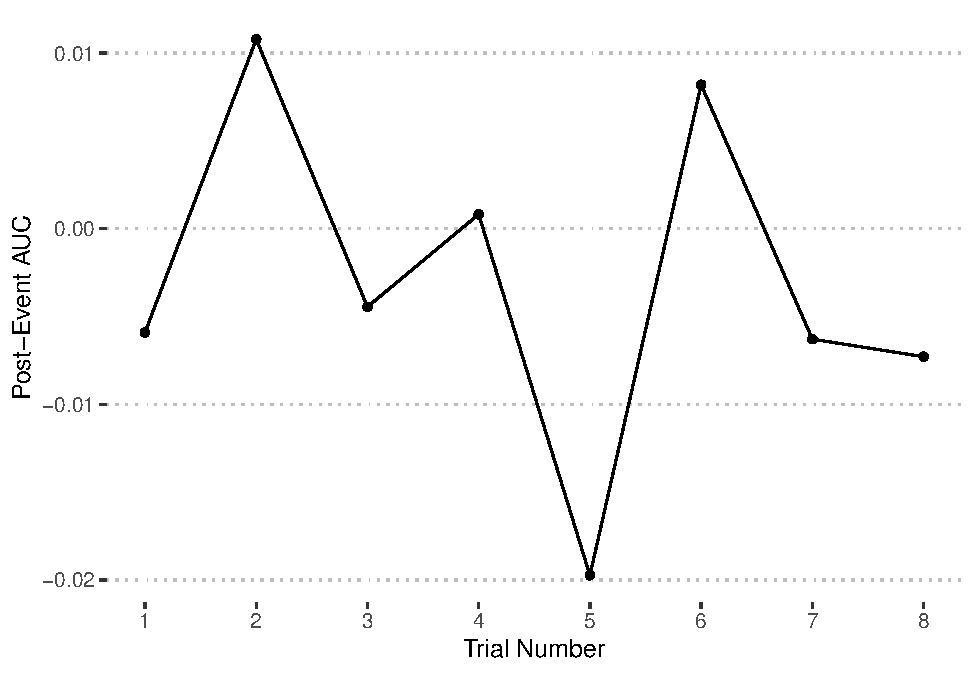
\includegraphics{fluoR_bookdown_files/figure-latex/unnamed-chunk-56-1.pdf}

\hypertarget{analysis-app-auc-ex2}{%
\subsubsection{Example 2}\label{analysis-app-auc-ex2}}

Compare pre- vs.~post- event activity for trials 1-8

This is a bit tricker. If you are comparing a baseine period to a post-event period, it will likely no longer be appropriate to use baseline deviations in transforming values for the full time series - at least when using the AUC.

This is because fluctuations in fluorescence on one side of the event (baseline) will be around the same, while post-event deviations from the norm will be exaggerated; causing a higher AUC.

With that in mind, let's do a typical z-score transformation for this data. Since each trial is measured for 4 seconds before event onset and 4 seconds after, \texttt{baseline\_transform} for the full 8-second period will result in the same thing as manually calculating z-scores for each trial.

\begin{Shaded}
\begin{Highlighting}[]
\CommentTok{### Format & standardize data}
\NormalTok{df <-}\StringTok{ }\KeywordTok{format_data}\NormalTok{(GCaMP)}

\NormalTok{df.stand <-}\StringTok{ }\NormalTok{fluoR}\OperatorTok{::}\KeywordTok{baseline_transform}\NormalTok{(}\DataTypeTok{dataframe =}\NormalTok{ df,}
                                      \DataTypeTok{trials =} \DecValTok{1}\OperatorTok{:}\DecValTok{8}\NormalTok{,}
                                      \DataTypeTok{baseline.times =} \KeywordTok{c}\NormalTok{(}\OperatorTok{-}\DecValTok{4}\NormalTok{,}\DecValTok{4}\NormalTok{), }\CommentTok{# or min-max timestamps}
                                      \DataTypeTok{type =} \StringTok{'z_standard'}\NormalTok{)}
\end{Highlighting}
\end{Shaded}

\begin{Shaded}
\begin{Highlighting}[]
\CommentTok{### Compute AUC values and create new data frame}
\NormalTok{auc.pre <-}\StringTok{ }\KeywordTok{auc_trials}\NormalTok{(}\DataTypeTok{dataframe =}\NormalTok{ df.stand, }\DataTypeTok{trials =} \DecValTok{1}\OperatorTok{:}\DecValTok{8}\NormalTok{,}
                      \DataTypeTok{time.range =} \KeywordTok{c}\NormalTok{(}\OperatorTok{-}\DecValTok{4}\NormalTok{,}\DecValTok{0}\NormalTok{))}
\NormalTok{auc.post <-}\StringTok{ }\KeywordTok{auc_trials}\NormalTok{(}\DataTypeTok{dataframe =}\NormalTok{ df.stand, }\DataTypeTok{trials =} \DecValTok{1}\OperatorTok{:}\DecValTok{8}\NormalTok{,}
                      \DataTypeTok{time.range =} \KeywordTok{c}\NormalTok{(}\DecValTok{0}\NormalTok{,}\DecValTok{4}\NormalTok{))}

\NormalTok{auc.df <-}\StringTok{ }\KeywordTok{data.frame}\NormalTok{(}
  \DataTypeTok{Trial =} \KeywordTok{rep}\NormalTok{(}\DecValTok{1}\OperatorTok{:}\DecValTok{8}\NormalTok{, }\DataTypeTok{times =} \DecValTok{2}\NormalTok{),}
  \DataTypeTok{Value =} \KeywordTok{c}\NormalTok{(auc.pre, auc.post), }\CommentTok{# 8 values pre & 8 values post}
  \DataTypeTok{Period =} \KeywordTok{rep}\NormalTok{(}\KeywordTok{c}\NormalTok{(}\StringTok{'pre'}\NormalTok{, }\StringTok{'post'}\NormalTok{), }\DataTypeTok{each =} \DecValTok{8}\NormalTok{)}
\NormalTok{)}
\end{Highlighting}
\end{Shaded}

We could graph some form of line or bar graph comparison

\begin{Shaded}
\begin{Highlighting}[]
\CommentTok{### Graphing}
\KeywordTok{ggplot}\NormalTok{(auc.df) }\OperatorTok{+}
\StringTok{  }\KeywordTok{geom_point}\NormalTok{(}\KeywordTok{aes}\NormalTok{(}\DataTypeTok{x =}\NormalTok{ Trial, }\DataTypeTok{y =}\NormalTok{ Value,}
                 \DataTypeTok{color =}\NormalTok{ Period, }\DataTypeTok{group =}\NormalTok{ Period)) }\OperatorTok{+}
\StringTok{  }\KeywordTok{geom_line}\NormalTok{(}\KeywordTok{aes}\NormalTok{(}\DataTypeTok{x =}\NormalTok{ Trial, }\DataTypeTok{y =}\NormalTok{ Value,}
                \DataTypeTok{color =}\NormalTok{ Period, }\DataTypeTok{group =}\NormalTok{ Period)) }\OperatorTok{+}
\StringTok{  }\KeywordTok{scale_x_continuous}\NormalTok{(}\DataTypeTok{breaks =} \DecValTok{1}\OperatorTok{:}\DecValTok{8}\NormalTok{) }\OperatorTok{+}
\StringTok{  }\KeywordTok{labs}\NormalTok{(}
    \DataTypeTok{x =} \StringTok{'Trial Number'}\NormalTok{,}
    \DataTypeTok{y =} \StringTok{'AUC'}\NormalTok{,}
    \DataTypeTok{title =} \StringTok{"Comparing fluorescence between pre- and post- event periods"}
\NormalTok{  )}
\end{Highlighting}
\end{Shaded}

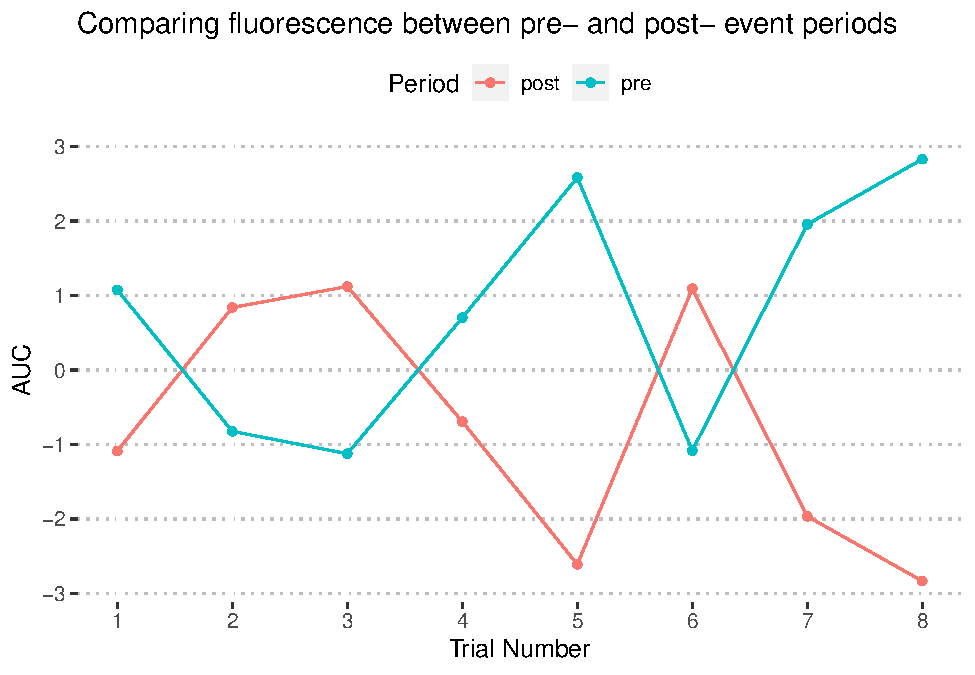
\includegraphics{fluoR_bookdown_files/figure-latex/unnamed-chunk-59-1.pdf}

Or we could subtract the values and graph the difference between pre- and post- trial AUC values. In other words, how much higher or lower is the post-trial AUC than the pre-trial AUC?

\begin{Shaded}
\begin{Highlighting}[]
\NormalTok{auc.diff <-}\StringTok{ }\NormalTok{auc.post }\OperatorTok{-}\StringTok{ }\NormalTok{auc.pre}

\NormalTok{auc.diffdf <-}\StringTok{ }\KeywordTok{data.frame}\NormalTok{(}
  \DataTypeTok{Trial =} \DecValTok{1}\OperatorTok{:}\DecValTok{8}\NormalTok{,}
  \DataTypeTok{Value =}\NormalTok{ auc.diff }\CommentTok{# 8 values pre & 8 values post}
\NormalTok{)}
\end{Highlighting}
\end{Shaded}

\begin{Shaded}
\begin{Highlighting}[]
\CommentTok{### Graphing}
\KeywordTok{ggplot}\NormalTok{(auc.diffdf) }\OperatorTok{+}
\StringTok{  }\KeywordTok{geom_point}\NormalTok{(}\KeywordTok{aes}\NormalTok{(}\DataTypeTok{x =}\NormalTok{ Trial, }\DataTypeTok{y =}\NormalTok{ Value)) }\OperatorTok{+}
\StringTok{  }\KeywordTok{geom_line}\NormalTok{(}\KeywordTok{aes}\NormalTok{(}\DataTypeTok{x =}\NormalTok{ Trial, }\DataTypeTok{y =}\NormalTok{ Value)) }\OperatorTok{+}
\StringTok{  }\KeywordTok{scale_x_continuous}\NormalTok{(}\DataTypeTok{breaks =} \DecValTok{1}\OperatorTok{:}\DecValTok{8}\NormalTok{) }\OperatorTok{+}
\StringTok{  }\KeywordTok{labs}\NormalTok{(}
    \DataTypeTok{x =} \StringTok{'Trial Number'}\NormalTok{,}
    \DataTypeTok{y =} \StringTok{'Post-Event AUC'}\NormalTok{,}
    \DataTypeTok{title =} \StringTok{'Post-event change in AUC'}
\NormalTok{  )}
\end{Highlighting}
\end{Shaded}

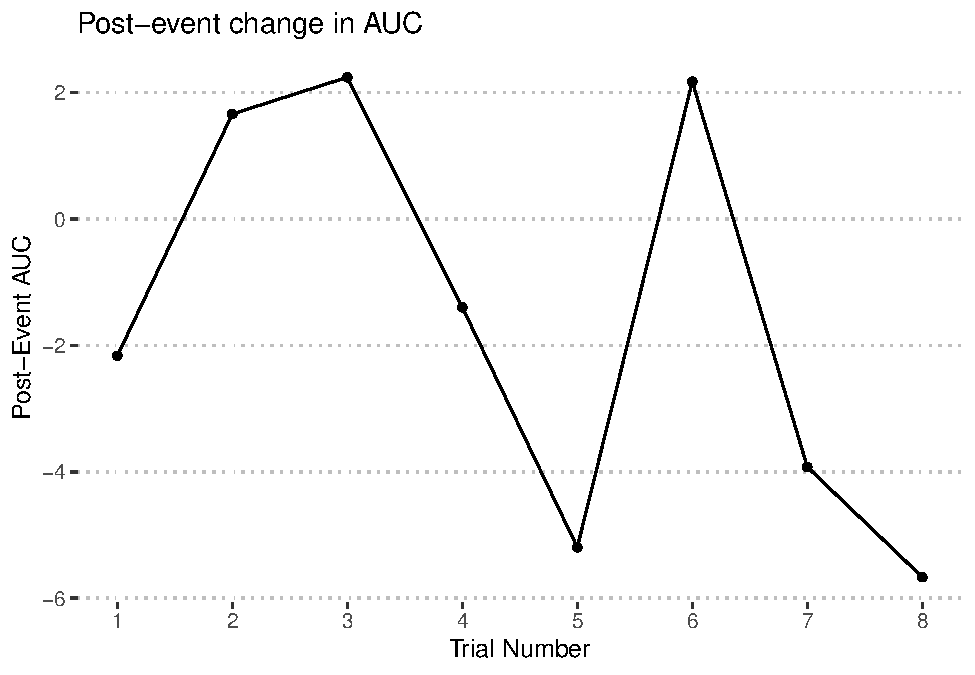
\includegraphics{fluoR_bookdown_files/figure-latex/unnamed-chunk-61-1.pdf}

On the other hand, it should still be okay to center at the baseline mean or median for interpretation purposes. This is because it is assumed that, after centering at baseline, the base line will hover around 0. Waves alternating above or below the 0-point on the y axis will mostly cancel each other out.

  \bibliography{references.bib}

\end{document}
